\documentclass[
    DIV=13,
    listof=totoc,
    bibliography=totoc,
]{tubaf-thesis}
\usepackage[sans]{tubaf-fonts}
\usepackage[footmark=author-subject]{tubaf-marks}
\usepackage{tubaf-logoext-faculty-five}

\usepackage[ngerman,english]{babel}

\usepackage[mode=match, separate-uncertainty=true]{siunitx}

\usepackage{graphicx}
\usepackage{subcaption}
\renewcommand*{\figureformat}{\figurename~\thefigure}
\renewcommand*{\tableformat}{\tablename~\thetable}

\usepackage{tabularray}
\UseTblrLibrary{booktabs}
\UseTblrLibrary{varwidth}
\UseTblrLibrary{amsmath}

\usepackage{enumitem}

\usepackage[sorting=none,style=numeric]{biblatex}

\addbibresource{refs.bib}
\usepackage{symbols}
\DeclareMathOperator{\sign}{sign}

\usepackage[hidelinks]{hyperref}
\usepackage[noabbrev]{cleveref}
\crefformat{pleq}{equations~(#2#1#3)}

\usepackage[record=nameref,abbreviations]{glossaries-extra}
\usepackage{glossaries}
\GlsXtrLoadResources[src=abbreviations]

\addtokomafont{chapterentry}{\normalfont\large}
\renewcommand\topfraction{0.9}
\renewcommand\bottomfraction{0.5}
\renewcommand\textfraction{0.1}
\renewcommand\floatpagefraction{0.85}

\renewcommand\emph[1]{\textcolor{darkgray}{#1}}

\usepackage{chemmacros}
\usepackage{todonotes}

\begin{document}
\title{Microscopic Simulation of Solid State Sintering Regarding Irregularly Shaped Powder Particles}
\author{Max Weiner}
\birthdate{22.03.1996}
\birthplace{Meißen}
\faculty{Fakultät für Werkstoffwissenschaft und Werkstofftechnologie\\der Technischen Universität Bergakademie Freiberg}
\date{\today}
\subject{Dissertation}
\currentdegree{Dipl.-Ing.}
\attaineddegree[Dr.-Ing.]{Doktor-Ingenieur}
\logo{\tubaflogoimf{2cm}{!}}

\selectlanguage{ngerman}
\maketitle

\selectlanguage{english}
\maketitle

\pagenumbering{arabic}

\tableofcontents

\input{tex/preface}

\addchap{Summary}\label{ch:summary}

\minisec{Deutsche Version}
Es wurde ein neuartiges Modell der Sinterung zweier bzw.~weniger Teilchen unter Verwendung scharfer Grenzflächen entwickelt und implementiert.
Die Anwendung des thermodynamischen Extremalprinzips erlaubt eine elegante und erweiterbare Formulierung.
Das numerische Verhalten des Modells unter Anwendung von Neuvernetzungsroutinen wurde untersucht und bewertet.
Es wurden Parameterstudien zu klassischen dimensionslosen Kenngrößen von Zweiteilchenmodellen, sowie asymmetrischer Material- wie Geometriepaarung durchgeführt, mit Literaturwissen abgeglichen und erklärt.
Kontakte mehrerer Teilchen wurden auf den Einfluss der Porenschließung untersucht, auch bei Anwesenheit inerter Teilchen.
Die Formcharakteristik von Pulverteilchen wurde unter statistischer Anwendung einer Formfunktion beschrieben und zur Generierung von Pulverteilchen als Eingabe in die Simulation verwendet.
Das mittlere Verhalten der zufällig generierten Teilchen wurde zur Beschreibung des Verhaltens des Pulvers genutzt und Unterschiede zu klassischen Verfahren der Mittelung diskutiert.

\minisec{English Version}
A novel model for the sintering of two or a couple of particles using sharp interfaces was developed and implemented.
The application of the thermodynamic extremal principle allows a concise and extendable formulation.
The numerical behavior of the model was investigated and evaluated under application of remeshing routines.
Parameter studies were conducted on classical dimensionless parameters of two-particle models, as well as asymmetric material and geometry pairing, which were compared with literature knowledge and explained.
Contacts between multiple particles were investigated for the influence of pore closure, even in the presence of inert particles.
The shape characteristics of powder particles were described using a statistical shape function and used to generate powder particles as input for the simulation.
The average behavior of the randomly generated particles was used to describe the behavior of the powder, and differences from classical averaging methods were discussed.


\part{Introduction}\label{part:introduction}
\chapter{Introduction to Sintering Technology}\label{ch:sintering-introduction}

The following elaborations on the basics of sintering are summaries from standard literature on the topic.
Some notable textbooks are those of \textcite{German1996, German2014}, \textcite{Geguzin1973}, \textcite{Kang2005}, \textcite{Exner1978}, \textcite{Fang2010}, \textcite{Rahaman2017} and \textcite{Routschka2017}.

Sintering in general is a process, in which compacted powders are densified and strengthened by the application of a heat treatment.
The actual mechanisms acting therein are discussed in \cref{sec:mechanisms}.
Sintering allows near-net shaping of possibly otherwise hard-to-shape materials, as well as creation of composites or alloys that are not produceible via the melt route.
To achieve required tolerances in geometry and material properties, a precise control and prediction of the density evolution (shrinkage) during the heat treatment is necessary.
In industrial practice, this is often done using empirical approaches, due to the complexity of the process (see \cref{sec:process-influences}),
Physical modeling, however, is required to improve understanding of mechanisms and observed effects and thereby allowing to design novel processing strategies and material concepts.
\cite{German1996}

\section{Process Steps for Manufacturing of Sintered Products}

\begin{figure}
    \includegraphics[width=\linewidth]{img/sintering_introduction/sintering_process_steps}
    \caption{Chart of Common Process Steps for Sintered Products}
    \label{fig:sintering_introduction/sintering_process_steps}
\end{figure}

The principal processing steps involved in manufacturing of sintered products shall be briefly discussed below.
\Cref{fig:sintering_introduction/sintering_process_steps} visualizes the process via a flow chart.

\begin{description}
    \item[Powder Mixing]
        Powders of differing particle size distribution, particle shape or even substance are mixed to achieve the desired sintering behavior and product properties.
        Optionally, additives facilitate compaction or achieve particular processing behavior (polymer resins, water, \ldots).
    \item[Compaction]
        The loose powder must be compacted to obtain a green body of sufficient density and strength.
        This can be accomplished by casting with or without vibrational assist, pressurized compaction, injection molding, or others.
        Usually, this step defines the desired shape of the product.
        Attention have to be paid to possible segregation of particles of distinct size or substance.
    \item[Sintering]
        The green body is heat treated to allow for diffusional processes, which are bonding the distinct powder particles together, and so achieve the desired strength and final density.
        During sintering the body usually shrinks in its dimensions, pore volume is reduced and the density increases due to internal volume displacement.
        If resin binders were used in the powder mixture, they have to be removed from the body by a low temperature heat treatment which pyrolyses and evaporates the binder, otherwise the component will crack during sintering due to fast gas formation which effects high stress.
        In some advanced processes, compaction and sintering is accomplished in one single step (pressure assisted sintering, field assisted sintering, \ldots).
    \item[Post-Processing] If required, the sintered body is machined to meet requested tolerances or surface properties. Porous parts for bearings are often infiltrated with lubricant.
\end{description}

In some cases, aggregate particles are formed by sintering simple bodies, crushing them, sieving the fragments and using them in mixing a novel powder for the actual component manufacturing.
This is used especially for refractory materials, where coarse grained microstructures are desirable for thermal shock resistance.
The aggregate particles are characterized by low internal sintering activity, so fresh active powder fractions have to be added to the mixture.
\cite{Routschka2017}

\section{Influencing Factors on Sintering Processes}\label{sec:process-influences}

The actual behavior of a sintering process is a complex problem, as there are many factors that influence the process and some of them are hard to describe or even quantify.
Most are interrelated.
They have been grouped to geometry, material and process related factors by \textcite{German2014}.
Below, the most important of these factors will be described, important interrelations are \emph{emphasized}.

\subsection{Geometric Factors}

These factors involve both the particle geometry and the geometry of the macroscopic sintering body.

\begin{description}
    \item[Particle Size]
        The particle size is the main geometric factor influencing sintering.
        Sintering is mainly driven by the reduction of energy bound in interfaces, either surfaces or grain boundaries.
        The mean particle size gives a rough estimate of the total energy bound in interfaces and thus of the available driving force.
        It also determines the length of diffusion paths and the required displaced volume to achieve a certain macroscopic response.
        The particle size determines the maximum achievable \emph{density} before sintering.
        Inhomogeneous size distributions aid to achieve high densities as pores can be filled by small particles.
    \item[Particle Shape]
        While \emph{particle size} affects the overall mean curvature of the particle, the local curvature and thus the driving force of sintering is determined by the actual shape of the particles.
        Shape deviations from ideal sphere let particles behave locally like larger or smaller ones in certain aspects.
    \item[Density and Porosity]
        The current relative density, or its inverse, the porosity, determines the still available volume reduction.
        With increasing density during sintering \emph{time}, the typical shape characteristic of pores changes from interconnected pore networks, to tube-like networks and finally isolated pores.
        The latter may be thermodynamically stable, especially when they are filled with gas due to trapped \emph{atmosphere}.
    \item[Neck Size]
        The current size of sinter necks (grain boundaries between particles) determine the mechanical strength of the body, the length of grain boundary diffusion paths, as well as the required volume to be displaced for certain shrinkage response.
        It also determines the available cross-section for inter particle mass flows.
    \item[Particle Packing]
        Depending on \emph{particle size} and \emph{particle shape} the packing may be more dense or loose and the coordination number of particle contacts changes.
        This affects \emph{density} and the mutual hindering of particles in their movement during sintering.
        Cracks may form due to inconvenient packings around diffusional inert particles.
\end{description}

\subsection{Material Factors}

These factors are related to the substance of the powder particles.

\begin{description}
    \item[Surface and Interface Energies]
        As the main driving force for sintering is the energy bound in interfaces, the energy per unit area in those interfaces plays a major role.
        Not only their absolute values, but also the ratio between distinct types of interfaces determines how the \emph{geometry} may evolve,
        as creation of a low-energy interface in favor of consuming a high-energy one may be thermodynamically beneficial.
    \item[Diffusivity]
        The advance of sintering in \emph{time} is heavily determined by the speed of the various diffusional processes acting (see \cref{sec:mechanisms}).
        Diffusional speed is dependent on the required activation energy and thus on \emph{temperature}.
        The ratio of the distinct mechanism's diffusivities affect the evolution and the final state of \emph{geometry}.
    \item[Vapor Pressure]
        A seldom encountered mechanism is evaporation/condensation of particle substance and transport via the gas phase (possibly with chemical reactions in reactive \emph{atmospheres}) as discussed in \cref{sec:mechanisms}.
        The actual vapor pressure at the respective \emph{temperature} determines the importance of this mechanism.
        Sometimes, only parts of the powder substance (impurities, specific alloying elements, binder resins) evaporate during the sintering process, which may change chemical composition, create defects in the microstructure or facilitate corrosion of the product (f.e.~zinc in brass).
    \item[Melting]
        Low-melting phases may be formed, which accelerate sintering and facilitate achievement of near-full density (liquid phase sintering) as the liquid is able to fill pores rapidly by viscous flow.
    \item[Flow Stress]
        In processes with high \emph{pressure}, plastic yielding may occur as an additional mechanism for \emph{densification}.
    \item[Crystal Structure]
        Depending on the crystal structure, material properties like \emph{surface and interface energies} and \emph{diffusivities} may be significantly anisotropic.
        This leads to non-spherical equilibrium \emph{particle shape}.
    \item[Chemical Interaction]
        Particles of different substance may be soluble or insoluble in each other, or may form new chemical substances through reactions.
        Concentration gradients within the particles or compound formation affects driving force and \emph{diffusivities}.
        Chemical interactions with the \emph{atmosphere} are often met.
\end{description}

\subsection{Processing Factors}

These factors describe the process setup.

\begin{description}
    \item[Temperature]
        The acting mechanisms are activated by elevated temperature to overcome their respective activation energy.
        Temperature determines the occurrence and speed of these mechanisms, as well as their relative importance.
        Key factors dependent on temperatures are the \emph{interface energies} and \emph{diffusivities}.
        In addition, temperature may activate several (maybe unwanted) side processes like \emph{melting}, chemical reactions with \emph{atmosphere} or affect \emph{chemical interaction} of different substances present.
    \item[Time]
        With advancing process time, the \emph{geometry} of the system evolves especially by increasing \emph{neck size} and \emph{density}.
        Time principally affects all conditions in the system as the state of the system evolves towards a lower energy configuration.
    \item[Pressure]
        Outer pressure on the compact during sintering acts as an additional driving force for \emph{densification} (pressure assisted sintering).
        Atmospheric pressure may act counter the \emph{vapor pressure}, thus inhibiting gas phase mechanisms.
    \item[Atmosphere]
        The surrounding atmosphere may cause \emph{chemical reactions} with the solid phase (especially oxidation).
        Gas adsorption affects surface \emph{diffusivities} and gas atoms may also diffuse through grain boundaries, possibly altering the interface properties or form new substances.
\end{description}

\chapter{Basic Theory of Sintering}\label{ch:basic-theory}

This chapter provides a brief overview of the basic theory of sintering, namely the mechanisms found in sintering processes, the mathematical treatment of those and the modelling of simple particle systems' evolution during sintering.

\section{Mechanisms of Sintering}\label{sec:mechanisms}

The following elaborations on the basic theory of sintering are based on standard literature for the topic. Some notable textbooks are those of \textcite{German1996, German2014}, \textcite{Geguzin1973}, \textcite{Kang2005} and \textcite{Exner1978}.

This work concentrates on solid state sintering, which means that there are no other than solid phases present in the system (exept the surrounding atmosphere).
Liquid phase sintering, where the material partially melts to assist closing pores, shall not be regarded.
Therefore, the term sintering shall always refer to solid state sintering from here on.

Sintering in general is a process, where powder material is densified and strengthened by thermal treatment at elevated temperatures.
The process is mainly driven by reduction of the energy stored in the system microstural features, such as grain boundaries, surfaces and other crystal defects.
These features are transformed by diffusional flows of material to reach a state of lower energy.
In this process, energy is dissipated, so it is an irreversible process.

\begin{figure}
	\centering
	% 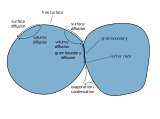
\includegraphics{img/introduction/state_of_the_art/diffusion_mechanisms}
	\caption{Schematic Overview of Diffusion Mechanisms Observed in Sintering Processes}
	\label{fig:introduction/state_of_the_art/diffusion_mechanisms}
\end{figure}

In common sintering processes the following diffusion mechanisms may occur, but their importance depends on powder geometry, process conditions and material properties.
The place and usual direction of their occurence is visualized in \autoref{fig:introduction/state_of_the_art/diffusion_mechanisms}.

\begin{description}
	\item[Volume Diffusion] Diffusion in the bulk material mediated by vacancies. Usually one of the slowest mechanisms and often neglegible.
	\item[Surface Diffusion] Diffusion along free surfaces (interfaces with surrounding atmosphere or vacuum). Much faster than volume diffusion.
	\item[Grain Boundary Diffusion] Diffusion along grain boundaries (solid-solid interfaces). Usually slower than surface diffusion but faster than volume diffusion.
	\item[Evaporation/Condensation] Evaporation of atoms to the gas phase and condensation at another point. Fast transport through the gas phase, but usually occurs only at very high temperatures or with very volatile substances.
\end{description}

Sintering is usually divided in three stages:

\begin{description}
	\item[Initial/Early Stage] Creation of initial contact. Major diffusion along surfaces to the sinter neck (triple points of surfaces and grain boundary). Rapid increase of neck size but low shrinkage.
	\item[Intermediate Stage] Porosity is still open and connected. Major diffusion along grain boundaries to the pores. Removal of substance at grain boundaries leeds to large shrinkage.
	\item[Final/Late Stage] Mainly closed porosity, gas pressure in pores may affect sintering. Still mainly grain boundary, but also volume diffusion. Slow progress in shrinkage and densification.
\end{description}



\section{Mathematical Description of Diffusion}\label{sec:diffusion}

The classic description of diffusional processes is done by Fick's laws \textcite{Fick1855}, which have the same mathematical form as the heat conduction laws by \textcite{Fourier1888}.
\autoref{eq:fick-first} shows Fick's first law for description of the diffusional flux $\Flux$ for the one-dimensional case.
It proposes a linear relationship between the concentration gradient and the flux.
For the concentration here the vacancy concentration $\VacancyConcentration$ is taken, as we assume only one diffusing species.
The flux of vacancies equals the negative flux of atoms.

\begin{equation}
    \Flux = - \DiffusionCoefficient \frac{\Deriv\VacancyConcentration}{\Deriv\X}
    \label{eq:fick-first}
\end{equation}

The diffusion coefficient heavily varies with temperature.
Its temperature dependence is usually described by an Arrhenius-type equation as in \autoref{eq:diffusion-coefficient-arrhenius} with a pre-exponential factor $\DiffusionCoefficient_0$ and the activation energy $\ActivationEnergy$.

\begin{equation}
    \DiffusionCoefficient = \DiffusionCoefficient_0 \exp \left( -\frac{\ActivationEnergy}{\GasConstant\Temperature} \right)
    \label{eq:diffusion-coefficient-arrhenius}
\end{equation}

The local vacancy concentration as driving force of the diffusion, however, depends on the thermal equilibrium vacancy concentration $\VacancyConcentration^\Standard$ and the local chemical potential $\ChemicalPotential$ as in \autoref{eq:vacancy-concentration}.

\begin{equation}
    \VacancyConcentration = \VacancyConcentration^\Standard \left( 1 - \frac{\ChemicalPotential - \ChemicalPotential^\Standard}{\GasConstant\Temperature} \right)
    \label{eq:vacancy-concentration}
\end{equation}

The main factor influencing the chemical potential in the regarded sintering processes are stresses, especially stresses originating from curved surfaces or interfaces (also known as surface tensions). The local chemical potential by a stress $\Stress$ is given as in \autoref{eq:potential-stress} with the molar volume $\MolarVolume$.

\begin{equation}
    \ChemicalPotential = \ChemicalPotential^\Standard + \Stress \MolarVolume
    \label{eq:potential-stress}
\end{equation}

The stress by a curved surface is given as in \autoref{eq:stress-surface-curvature} with the surface resp.\ interface energy $\InterfaceEnergy$ and the curvature $\Curvature$.

\begin{equation}
    \Stress = \InterfaceEnergy \Curvature
    \label{eq:stress-surface-curvature}
\end{equation}

Other stresses present affect the progress of sintering nevertheless.
The reason for pressure assisted sintering can directly be seen from these equations, since the applied pressure drives the diffusion from the inner of the grain boundaries to the necks.

In the triple point, where three interfaces meet, the dihedral angles between the interfaces $\DihedralAngle_i$ will follow Young's equation (\autoref{eq:youngs-dihedral}) in equilibrium with $\DihedralAngle_1 + \DihedralAngle_2 + \DihedralAngle_3 = 2\PI$,
where the $\InterfaceEnergy_i$ are the interface energies of the interface opposed to the angle with the same index.
\begin{equation}
    \frac{\InterfaceEnergy_1}{\sin \DihedralAngle_1} = \frac{\InterfaceEnergy_2}{\sin \DihedralAngle_2} = \frac{\InterfaceEnergy_3}{\sin \DihedralAngle_3}
    \label{eq:youngs-dihedral}
\end{equation}
This is equivalent to a triangle with side lengths $\InterfaceEnergy_i$ and the respective opposite angles $\PI - \DihedralAngle_i$ \cite{Hoffman1972}.
From this can directly be seen, that the sum of either two surface energies must be larger than the third, or this triangle does not exist and \autoref{eq:youngs-dihedral} can not be solved.
The non-existence of the triangle implies that such a junction can never be in equilibrium, if no other forces on the junction are present (like pinning forces) \cite{King1999}.
So in this case, it is always beneficial from energetic point of view to consume the boundary with the largest interface energy while enlarging the others.

\section{Non-Equilibrium Thermodynamics}\label{sec:thermodynamics}

Sintering processes are by their nature non-equilibrium thermodynamical processes which drive the system state towards an equilibrium state.
The major problem of non-equilibrium thermodynamics is that the common thermodynamical quantities temperature and entropy are only defined in equilibrium state.
Therefore, the second law of thermodynamics (entropy must always increase) only holds for transitions between equilibrium states and may thus not describe the pathway between these states, but only the whole step as one.
To circumvent this problem, several approaches have been developed, from which the \gls{CIT} (sometimes referred to as \gls{TIP}) and the thermodynamics of \gls{IVS} shall be discussed here in particular.
The following elaborations are based on textbooks of \textcite{deGroot1962, Maugin1999, Lebon2008} and a review article of \textcite{Maugin1994}.

\subsection{Classical Theory of Irreversible Thermodynamics}

A non-equilibrium state is characterized by inhomogeneity and thus gradients of its major state variables.
The central assumption of the classic treatment of non-equilibrium irreversible processes is that of a local equilibrium.
It is postulated that in a certain small volume of the system, the equilibrium state is present despite the gradient to the next neighboring volume.
This means that the characteristic time of local equilibration is much smaller than the characteristic time of the macroscopic process, expressed by the Deborah number $\DeborahNumber = \TimeNorm_{\text{local}} / \TimeNorm_{\text{global}} << 1$.
The volume cell must be small enough to fulfill this timescale condition, but large enough to be described sufficiently well as a continuum.
The time needed for restoration of a local equilibrium state can be neglected in comparison to the macroscopical evolution of the system.
This allows to grant the usual meaning to temperature and entropy.
On the other hand, processes with a Deborah number $\DeborahNumber >> 1$ can be regarded as quasi-static.
Those assumptions hold true for most thermodynamical processes in question, especially for the here regarded sintering.
So, the irreversible process reduces to a sequence in time of local equilibria.

The system's state at a certain point in time is defined by the vector of state variables $\ExternalStateVariable$.
As sintering is a process at constant temperature and pressure, the thermodynamic condition of equilibrium is to be formulated in terms of Gibbs' energy $\GibbsEnergy(\ExternalStateVariable)$, which is a function of the state.
Temperature can be assumed constant, as the energy dissipated is small compared to the thermal energy stored in the system (sintering body and surrounding furnace), so the system does not heat up significantly.
Temperature changes during the process are external changes to the system and not due to its internal evolution.
Conventional sintering processes are conducted under constant atmospheric pressure, whereas in pressure-assisted sintering the applied pressure is usually kept constant by control.

The thermodynamic forces driving the evolution of the system are given as the partial derivatives of Gibbs' energy with respect to the state.
The gradient of the Gibbs' energy equals zero, when the system has reached equilibrium.
\begin{equation}
    \frac{\partial \GibbsEnergy}{\partial \Vect\ExternalStateVariable} = 0
    \label{eq:cit-gibbs-equilibrium}
\end{equation}

Changes in the state variables are obtained by the occurrence of respective fluxes $\Vect\Flux$.
The dissipation $\Dissipation$ during evolution of the system is proportional to the product of the fluxes and their respective thermodynamic forces.
\begin{equation}
    \Dissipation \sim \frac{\partial \GibbsEnergy}{\partial \Vect\ExternalStateVariable} \cdot \Vect\Flux \ge 0
    \label{eq:cit-dissipation}
\end{equation}

A usual (and for many processes valid) assumption is linearity between the fluxes $\Vect\Flux$ and the thermodynamic driving forces $\frac{\partial \GibbsEnergy}{\partial \Vect\ExternalStateVariable}$ with a coefficient $\Vect{C}$.
This corresponds to the empirical description of diffusion by Fick's law (\cref{eq:fick-first}).
\begin{equation}
    \Vect\Flux = \Vect{C} \cdot \frac{\partial \GibbsEnergy}{\partial \Vect\ExternalStateVariable}
    \label{eq:cit-flux-force-relationship}
\end{equation}

\subsection{Internal Variables of State}\label{subsec:internal-variables-of-state}

As the microscopic nature of thermodynamical systems is often too complex to be described alone by the macroscopical observable and controllable \glspl{EVS} $\Vect\ExternalStateVariable$ (such as temperature, pressure, internal energy and entropy), approaches only considering those neglect large amounts of internal processes and specifics of the state.
An approach applied enormously successfully is that of the introduction of \glspl{IVS} $\Vect\InternalStateVariable$ which represent dissipative quantities in the system and can be freely chosen dependent on the desired precision and particularity of the model.
In contrast to external variables of state, which define the macroscopic response of the system and are thus relatively easy to measure and control, internal variables of state may be measurable, but are usually out of control when setting up an experiment.
The approach was mainly developed by authors like \textcite{Bataille1979}, \textcite{Kestin1990, Kestin1992}, \textcite{Muschik1990} and \textcite{Maugin1994, Maugin1994a}.
\textcite{Maugin2015} gives an extensive review and history.

The formalism axiomatically associates a local accompanying equilibrium state dependent on the local non-equilibrium \glspl{EVS} and the \glspl{IVS} to a volume cell at a respective point in time.
This is an extension of the former assumption of local equilibrium in \gls{CIT}.
The local change in Gibbs' energy is then given by:
\begin{equation}
    \Deriv\GibbsEnergy = \frac{\partial \GibbsEnergy}{\partial \Vect\ExternalStateVariable} \cdot \Deriv\Vect\ExternalStateVariable + \frac{\partial \GibbsEnergy}{\partial \Vect\InternalStateVariable} \cdot \Deriv\Vect\InternalStateVariable
    \label{eq:ivs-local-las-gibbs-derivative}
\end{equation}

The physical meaning and applicability of this system to describe the real process highly depends on the choice of the \gls{IVS}.
Principally, one is free to choose the internal variables depending on requirements on precision, model depth and computational effort.
However, they must fulfill some conditions to be appropriate.
Similar to the requirements of local equilibrium in \gls{CIT}, an \gls{IVS} can be considered to always have their local equilibrium value if $\DeborahNumber << 1$ holds.
On the other hand, if $\DeborahNumber >> 1$, the variable can be assumed constant in regard to the equilibrium condition.
If neither is valid, the variable is considered to be a bad choice and another one should be selected to describe the internal state.

Another important type of variables in this notion is that of \glspl{IDF}, which are not of pure dissipative nature.
They show relevant inertia within the respective timescale, which is equivalent to $\DeborahNumber \approx 1$.
\glspl{IDF} must be accompanied by their own kinetic law in terms of a differential equation to be included in the simulation.
They may, but do not have to, include a dissipative contribution as \gls{IVS} do.

A numerical approach to obtain a system of ordinary differential equations from this formalism will be discussed in \cref{sec:extremal-principle}.

\section{Simplified Quantitative Descriptions of Sintering Processes}\label{sec:simple-solutions}

The mathematical description of diffusion phenomena based on potentials and empirical kinetic diffusion coefficients as discussed in \cref{sec:diffusion} does not encounter major difficulties.
The real complexity of modelling sintering processes arises in the geometrical state and evolution of the system.
Early models on particle level therefore imposed heavy assumptions on the geometry of the initial particles and of the sinter neck, to be able to obtain a concise and efficient formulations.
This was especially required as powerful computer systems were not available.
Such models shall be regarded in this section, more advanced approaches, however, are regarded in \cref{ch:numerical-methods}.

The most common simplification applied is the assumption of a circular (2D) or spherical (3D) geometry of the particles before sintering.
This has the following main benefits:
\begin{itemize}
    \item Simple characterization of particles using a single parameter (radius or diameter).
    \item Absence of diffusional flows on large parts of the particle surface due to constant curvature, the only gradients are present near the neck.
    \item Symmetry of the particle contact with respect to the approaching axis and thus also invariance of particle rotation.
\end{itemize}
Such a system's state is sufficiently described by the radii of the involved particles, their distances (or positions) and the current size of the necks between the particles.
Often, only a single pair of particles of the same size and material properties is regarded, which introduces another degree of symmetry.

These simplifications allow the analytical solution of the governing differential equations and lead to equations of the type in \cref{eq:inital-stage-neck-size} for neck radius and \cref{eq:inital-stage-shrinkage} for shrinkage.
Therein, $\Time$ denotes the sinter duration, $\NeckRadius$ the neck radius, $\Radius_{\Particle}$ the particle radius and $B$, $m$ and $n$ are parameters depending on the acting transport mechanisms.
Notable examples of such models are given by \textcite{Kuczynski1949, Johnson1963, Kingery1955, Coblenz1980, German2017}.
\begin{align}
    \left( \frac{\NeckRadius}{\Radius_{\Particle}} \right)^n &= \frac{B \Time}{\left( 2 \Radius_{\Particle} \right)^m}
    \label{eq:inital-stage-neck-size}\\
    \Shrinkage^n &= \frac{B \Time}{\left( 2 \Radius_{\Particle} \right)^m}
    \label{eq:inital-stage-shrinkage}
\end{align}

A common result from these models, alongside with dimensionless parameter studies, is the definition of the dimensionless timescale for two-particle-sintering processes as given in \cref{eq:normalized_time}.
Often the surface energy $\InterfaceEnergy_{\Surface}$ and surface diffusion coefficient $\DiffusionCoefficient_{\Surface}$ are referenced, but the equal is possible using the properties of the grain boundary.
\begin{equation}
    \Normalized\Time = \frac{\MolarVolume\VacancyConcentration^\Standard\DiffusionCoefficient_{\Surface}\InterfaceEnergy_{\Surface}}{\GasConstant\Temperature\Radius_{\Particle}^4} \cdot \Time
    \label{eq:normalized_time}
\end{equation}

Similar treatments have been given for the intermediate and final stages of sintering.
In these stages the particles are usually assumed as polyhedra with cylindrical or spherical pores on the boundaries.
Since these stages are mainly characterized by the decrease in pore volume, they are formulated in terms of densification.
Examples for such models are \textcite{Coble1961a}, \textcite{Swinkels1981}, \textcite{Kang2004} and \textcite{Gouvea2024}.

The predictive value of such simple solutions is rather low because of their heavy simplifications, but they can be used to create empirical fits on experimental data.


\chapter{Numerical Methods for Sintering Simulation}\label{ch:numerical-methods}

Sintering models can be distinguished in two main branches: macroscale and microscale models. 
The former regard the porous worpiece material as a continuum with variable density. 
Stresses and strains are usually modelled using visco-plastic material laws or similar while the density evolves during thermal treatment or plastic deformation (mechanical compaction). 
Numerical solution are commonly obtained by use of the \gls{FEM}.
The focus of these models usually lies in the analysis of density, strain and stress distributions, as well as damage estimation, in a component with often complex geometry.
Examples for these models are found in \textcite{Olevsky1998, Safonov2019, Kraft2004, Al-Qudsi2014, Shi2023}. 
These models will not be considered in the following, as this work concentrates on the second kind.

Microscale models regard the interaction between distinct grains resp. powder particles and the evolution of their interfaces to each other and the environment. 
The solution space typically includes from two to a limited number of distinct particles or a defined \gls{RVE}. 
Physics-based models model the distinct diffusion mechanisms occuring and their effect on the particle and/or pore shape. 

There are basically two ways of representing the interfaces of particles to each other or the environment: sharp and diffuse interfaces. 
Both were reported to be used in sintering simulation before.

A sharp interface means that there is a defined line were the interface is supposed to be located, on one side the one phase, on ther other side the other, without any transition.
Sharp interfaces are the most straightforward approach, as most people are used to think in that way, although in reality, interfaces have a non-zero width, typically in the scale of a few atom diameters. 
One may think about the adsorption and diffusion layer on solid surfaces or the mislalignment voids between crystallites in grain boundaries. 
However, the width of interfaces is usually much smaller then the size of particles or microscopic surface features, and can therefore be neglected.
Sharp interfaces can be described directly by the coordinates of their line string, either as a linear or non-linear spline or similar, or, by following an equality condition in the solution space (e.g. level-set method or cellular automata).
The curvature of such an interface can directly be calculated by interpolation of its coordinates, f.e. for use in \autoref{eq:stress-surface-curvature}.
Models of this type are discussed in detail in \autoref{sec:sharp-interfaces}. 

A diffuse interface means that there is a certain region of transition between the two phases.
The most common approach for that is the phase field method, where the phase present at a point is defined by the value of one or multiple auxiliary variables, whose values go smoothly between \num{0} and \num{1}.
For illustration purposes the interface is often defined at a ceratin threshold value of the phase field variables, but the model usually does not work with such, but only with the gradient of the variable.
There are no hard transitions in such models, but everything is smooth (except for the limitations of numerical discretization).
Models of this type are discussed in detail in \autoref{sec:diffuse-interfaces}.

\section{Interface Descriptions}\label{sec:interfaces}

\begin{figure}
    \begin{center}
        \includegraphics[width=0.95\textwidth]{img/numerical_methods/classification}
    \end{center}
    \caption{Classification of Interface Description Methods}\label{fig:classification}
\end{figure}

Since the tracking of the interfaces is a key problem in modelling of sintering, the numerical methods shall be classified by this feature.
See \cref{fig:classification} for a visualization of this classification.
The approach taken there is also crucial for the used numerical integration procedure, the required material data and the reliability of the obtained simulation results.

The first distinction can be made into approaches with direct and indirect interface tracking.
Direct tracking means that the location of the interface is directly defined by discrete points in space, which are moved during the integration procedure to describe the shape evolution of the interface.
So in this family of approaches there is a sharp interface definition.
A sharp interface means that the interface is considered as a defined line, where the two phases exist on the one resp.~the other side of the line.
The curvature of such an interface can directly be calculated by interpolation of its coordinates, for example to be used in \cref{eq:stress-surface-curvature}.
Direct interface approaches usually use the \glsfirst{FDM} or the \glsfirst{FEM} to represent the particle shape.

Indirect tracking, however, means that the interface location is defined by the value of an auxiliary function.
The discretization is there connected to the solution space, the points are fixed in space and the motion of the interface is just realized by changes in the auxiliary function values.
Indirect interface methods can further be classified in methods with sharp and diffuse interfaces.
Approaches with a sharp interface definition include the \glsfirst{LSM} (see \cref{subsec:interfaces-level-set}) and \glsfirstplural{CA} (see \cref{subsec:interfaces-cellular-automata}) approaches.

Diffuse interfaces mean a more or less smooth transition between two phases, so that the actual position can not directly be located.
This diffusivity must not be confused with the physical width of the interface.
The physical width of the interface is the region where the atomic structure significantly deviates from the bulk structure.
This is usually in the order of a few atomic diameters (around or below \qty{1}{\nano\meter}).
The width of a diffuse interface is a numerical artifact and depends on the size of the spatial discretization.
Typical widths are here rather in the range around \qty{1}{\micro\meter}.
The diffuse interface width is not physical, but a numeric requirement to be able to calculate gradients through the interface.
Diffuse interfaces are used in \glsfirst{PFM} approaches (see \cref{subsec:interfaces-phase-field}).

\subsection{Direct Interface Approaches}\label{subsec:interfaces-direct}

Several authors have published sintering models where the interfaces are described directly by discrete points either in a finite difference or finite element scheme.

This approach has the great advantage of direct and easy computation of geometrical features such as curvatures, as the defining points are directly available.
Curvature calculation is either done by application of finite differences~\cite{Svoboda1995, Bouvard1996} or by interpolation functions~\cite{Svoboda1995, Nikolic1999, Jagota1988a, Lechelle2014}.

The major problem of direct interface approaches is maintaining the contact conditions resp.~the geometric validity of the grain boundary.
Most models, therefore, assume a heavily idealised (planar) grain boundary and rely on symmetry to simplify determination of the particle motions~\cite{Svoboda1995, Svoboda1992, Bouvard1996, Jagota1988a, Wakai2018}.
The problem therefore reduced to determining the evolution of the surface geometry.

\textcite{Svoboda1995, Bouvard1996} are classic \gls{FDM}-based solutions of two equal circular particles with heavy symmetry assumptions.
An advanced \gls{FDM}-based model was published by \textcite{Klinger2013, Klinger2012, Klinger2011} which supports curved grain boundaries.

\textcite{Jagota1988a} published a direct FE model for two-particle sintering, however, based on viscous constitutive equations.
So this is merely feasible for amorphous materials rather than crystalline ones.
\textcite{Lechelle2014} built a direct FE model in the tradition of classic mechanical FE approaches.
It regards surface and grain boundary diffusion considering the interfacial stresses as outer load and applying contact conditions in the grain boundary.
This model appears to be basically able to work with particles of arbitrary shape, but was only evaluated for two spherical particles.

There is a free and open-source program by \textcite{Brakke1992} aimed at modelling the evolution of different surfaces in time by minimizing the energy stepwise.
However, it lacks direct support for time-coupled simulation, as the kinetics are solely determined by use of a global constant.
\textcite{Wakai2022} recently built a 3D multiple-particle sintering simulation based on this program, an older version of the approach is published in \cite{Wakai2011, Wakai2018}.
Their implementation includes rigid body motion only for symmetric cases, as all motion is directed towards the center point.

\subsection{Indirect Sharp Interface Approaches Using the Level-Set Method}\label{subsec:interfaces-level-set}

Tracking of interfaces using a sharp interface is possible by application of the \gls{LSM}.
An auxiliary function (or level-set function) $\phi$ is introduced which is positive inside the regarded phase and negative outside, so $\phi = 0$ defines the location of the interface.
Usually the value of the function corresponds to the signed euclidic distance of the current point from the boundary.
This enables the use of the gradient $\nabla \phi$ for example for calculation of the interface curvature.
The time evolution of the auxiliary function is described by \cref{eq:level-set-elementary}, with the interface velocity vector $\Vect v$.
\begin{equation}
    \frac{\partial\phi}{\partial\Time} = \Vect v \nabla\phi = 0
    \label{eq:level-set-elementary}
\end{equation}

Overview articles of the method in general were published for example by \textcite{Osher2001, Gibou2018, vanDijk2013}.
Applications to sintering problems have been conducted by \textcite{Bruchon2010, Bruchon2012, PinoMunoz2013}.
The basic approach is very similar to direct interface approaches, as diffusional fluxes are directly computed by application of Fick's law with potentials obtained from surface curvature.
The velocity $\Vect v$ is taken normal from the current surface and calculated from mass conservation incorporating the diffusional fluxes.
The curvature is obtained from the gradient of the level-set function by \cref{eq:level-set-curvature}.
\begin{equation}
    \Curvature = \nabla \cdot \frac{\nabla\phi}{\Abs{\nabla\phi}}
    \label{eq:level-set-curvature}
\end{equation}

The solution of \cref{eq:level-set-elementary}, however, is usually only conducted in a certain region near the interface.
Outside this region the solution is roughly approximated, but this does not preserve the signed distance character of the level-set function.
For this reason, a renormalization procedure is applied to restore this character.

Level-set approaches give a clean indirect description of a sharp interface.
This approach circumvents the logical problems inherent in diffuse interfaces, gives a smooth interface line in contrast to cellular approaches (\cref{subsec:interfaces-cellular-automata}) and nevertheless has the advantage of easy indirect interface tracking.
The main disadvantage of this method is the restriction to only two phases, at least no extension to multiple phases has been published yet.
This is likely the main reason, why the adoption of this method for sintering problems is currently rather low.
Especially, there is no numeric distinction between the particles, just between solid and void.
Therefore, also the boundary between the particles is inexistent, so grain boundary diffusion cannot be described.

\subsection{Indirect Sharp Interface Approaches Using Cellular Automata}\label{subsec:interfaces-cellular-automata}

A \gls{CA} is a discretization scheme, where the solution space is discretized in finite cells, of possible arbitrary shape.
The state of these cells (or sometimes voxels), for example the belonging to a phase or grain, is defined by discrete state variables.
In each time step the state variables' values are changed in dependence on the governing model equations.
For sintering, these governing equations are usually randomized, which leads to the \glsfirst{kMCM}, which will be discussed in \cref{subsec:monte-carlo-kinetic-sintering}.
In this type of model there is usually no continuous or almost continuous interface, as the interface is just the outer boundary of coherent cells belonging to the same phase or grain.
This can be imagined as a low resolution pixel graphic with discrete colors.

\subsection{Indirect Diffuse Interface Approaches Using the Phase Field Method}\label{subsec:interfaces-phase-field}

The phase field method is based on the idea to describe the phase distribution in a regarded solution space by the value of an auxiliary variable, usually referred to as phase field variable or order parameter.
The task of tracking the interface is reduced to the task of describing the time evolution of the order parameter by use of differential equations.
There are several excellent review articles on basics and application of the \gls{PFM}~\cite{Chen2022, Qin2010, Chen2002, Steinbach2009, Steinbach2013, Wang2010, Tonks2019}.

The method resides on a grand energy potential, either written in terms of Gibbs energy $\GibbsEnergy$ or Helmholtz energy $\HelmholtzEnergy$, which describes the thermodynamic evolution of the system.
For the example of a coupled thermal and diffusional system consisting of two phases, the total differential of the specific Helmholtz free energy $\SpecificHelmholtzEnergy$ can be stated as \cref{eq:phase-field-helmholtz-functional}, with the specific entropy $\SpecificEntropy$, the temperature $\Temperature$, the chemical potential $\ChemicalPotential$ and concentration $\Concentration_i$ of species $i$, as well as the order parameter for the phase $\xi$ and the thermodynamic driving force of phase transition $\beta$, which includes both the driving force of bulk transformation and of interface generation or destruction.
\begin{equation}
    \Deriv f = - \SpecificEntropy \Deriv \Temperature + \ChemicalPotential_i \Deriv \Concentration_i - \beta \Deriv \xi
    \label{eq:phase-field-helmholtz-functional}
\end{equation}

According to \textcite{Allen1979} the driving force $\beta$ is given as in \cref{eq:allen-cahn-driving}, which includes a dependency on the gradient of the order parameter $\xi$, which covers the change in energy due to change in interfacial areas.
$\kappa_\xi$ is a material dependent parameter (gradient coefficient), which is related to the interface energy $\InterfaceEnergy$.
\begin{equation}
    \beta = - \left( \frac{\partial\SpecificHelmholtzEnergy}{\partial\xi} - \kappa_\xi \nabla^2 \xi \right)
    \label{eq:allen-cahn-driving}
\end{equation}

Assuming kinetics proportional to the driving force (as usual for small driving forces), \cref{eq:allen-cahn-differential} as evolution presription for the order parameter is obtained with $M_\xi$ as kinetic constant (mobility constant).
\begin{equation}
    \frac{\Deriv\xi}{\Deriv\Time} = \Mobility_\xi \beta = -\Mobility_\xi \left( \frac{\partial\SpecificHelmholtzEnergy}{\partial\xi} - \kappa_\xi \nabla^2 \xi \right)
    \label{eq:allen-cahn-differential}
\end{equation}

The width of the interface can be estimated using \cref{eq:phase-field-interfacial-width}.
To ensure numerical stability and accuracy, the discretization width of the numerical solution should be smaller than the interface width (at least four cells within the interface according to \textcite{Qin2010}).
\begin{equation}
    l = \sqrt{\frac{2\kappa_\xi \xi_\Equilibrium}{\SpecificHelmholtzEnergy(\xi) - \SpecificHelmholtzEnergy(\xi_\Equilibrium)}}
    \label{eq:phase-field-interfacial-width}
\end{equation}

For conserved order parameters, the Cahn-Hillard equation \cite{Cahn1961} can be applied instead as given in \cref{eq:cahn-hillard}.
\begin{equation}
    \frac{\Deriv\xi}{\Deriv\Time} = \nabla \cdot \Mobility_\xi \nabla \left( \frac{\partial\SpecificHelmholtzEnergy}{\partial\xi} - \kappa_\xi \nabla^2 \xi \right)
    \label{eq:cahn-hillard}
\end{equation}

Additional kinetic equations are required for the other state variables $\Temperature$ and $\Concentration_i$.
Temperature kinetics are usually described by \cref{eq:phase-field-kinetic-temperature} with the specific heat capacity $c_\Volume$ and the heat conductivity $k$, which is in fact just Fourier's heat conduction law.
Diffusion kinetics, however, can be described by \cref{eq:phase-field-kinetic-concentration} with a law similar to the classic description of diffusion using Fick's law (see \cref{sec:diffusion}).
Note that the mobility coefficient $\Mobility_{ij}$ is here not identical to the diffusion coeffcient $\DiffusionCoefficient$, since it relates the flux to the gradient of chemical potential $\ChemicalPotential$, instead of the concentration gradient.
These common laws are in fact just special cases of the Cahn-Hillard (\cref{eq:cahn-hillard}) equation, as both are conserved fields.
\begin{equation}
    \frac{\Deriv\Temperature}{\Deriv \Time} = \frac{1}{c_\Volume} \nabla \cdot \left( k \nabla \Temperature \right)
    \label{eq:phase-field-kinetic-temperature}
\end{equation}
\begin{equation}
    \frac{\Deriv\Concentration_i}{\Deriv \Time} = \nabla \cdot \left( \Mobility_{ij} \nabla \ChemicalPotential_j \right)
    \label{eq:phase-field-kinetic-concentration}
\end{equation}

The phase field method offers a flexible approach to the description of heterogeneous thermodynamic systems, as additional energy contributions can be included easily as additonal terms in the energy functional \cref{eq:phase-field-helmholtz-functional}.
Additional phases can be included by introduction of additional order parameters.
Additional internal processes like chemical reactions can be regarded in the same way.
The numerical treatment of all state variables in the system is very similar, the only important distinction is the for conserved fields (e.g. concentrations) and non-conserved fields (e.g. phase variables).
Numerical difficulties occur due to the varying magnitude of the involved gradients.
Influence of crystal orientation can also be introduced into the system by directionally dependent material parameters~\cite{Deng2012}.
For sintering problems the influence of temperature gradients is usually neglected, except for \textcite{Yang2020}.
Today, the \gls{PFM} is the most used approach for simulation of sintering, but also applied in other fields of materials modelling and beyond.
The main reason for this appears to be its flexibility and clean and easy formulation of multiple coupled mechanisms.

The main disadvantage of phase field models is the unphysical wide interface caused by the continuous description of phase composition by the order parameters.
Therefore, material parameters in energy and kinetic functions are not directly identifiable with actual physical quantities.
They depend not only on the actual material properties, but also on the numerical properties of the model, such as interface width and discretization width.
The local characteristics of the (approximately) sharp real interface must be transformed to the diffuse interface while maintaining the globally observable behavior.
Applications of this method to sintering problems often target on general observations on sintering behavior far from any real material data~\cite{Deng2012, Wang2006, Asp2006, Jing2003, Kumar2010, Kumar2011, Shinagawa2014}.
\textcite{Biswas2016, Biswas2017} determined the mobilities $\Mobility$ from the corresponding diffusion coefficients by use of a method by \textcite{Moelans2008}.
Several authors~\cite{Chockalingam2016, Biswas2016, Biswas2017, Choudhuri2021} used an equation system developed by \textcite{Ahmed2013} to determine the gradient coefficients $\kappa$ and from actual material data, however still including the numerical properties.

A major difficulty in application to sintering problems is the description of rigid body motion.
For modeling dense microstructures, the only possible changes are due to phase transformations and diffusional flows, since the space is fully occupied by matter.
In sintering, however, there is usually a significant amount of void (or atmosphere), which is not able to withstand the motion of a solid body.
The distinct grains move relative to each other due to changes in their contact geometry effected by diffusional flows along the grain boundaries.
This is observed macroscopically as shrinkage, a main phenomenon of sintering processes.
The movement is not directly driven by diffusional flows or phase transformations, so it cannot be included directly in the grand energy functional.
Some phase-field-based sintering model neglect this mechanism, therefore not regarding the phenomenon of shrinkage \cite{Asp2006, Chockalingam2016, Hotzer2019, Jing2003, Kumar2010, Kumar2011, Deng2012, Zhang2014, Yang2020, Choudhuri2021}.

An approach by \textcite{Wang2006} (and adopted by others~\cite{Termuhlen2021, Biswas2016, Biswas2017}) regards the rigid body motion by additional terms in the Allen-Cahn and Cahn-Hillard equations including an advection velocity of the particles.
This advection velocity is calculated from the force and torque balance on the particle volume.
Forces and torques are obtained from the order parameter gradient.
\textcite{Shinagawa2014} used a coupled \gls{DEM} model to determine the rigid body motion independently from the phase field.
Both models are updated from the other by an iterational process.
\textcite{Ivannikov2021} introduced a grain boundary force similar to that of \textcite{Wang2006}, but did not include it in the kinetics equation, rather they set a constraint on it to be always zero.
If the constraint is violated, they calculate and apply an advection vector to restore it.

The underlying numerical method to solve the field equations is usually a \gls{FDM}~\cite{Wang2006, Hotzer2019, Jing2003, Kumar2010, Kumar2011, Zhang2014} or \gls{FEM}~\cite{Asp2006, Chockalingam2016, Biswas2016, Biswas2017, Greenquist2020, Ivannikov2021} scheme.
Most models are formulated in 2D, only a few in 3D space~\cite{Greenquist2020, Termuhlen2021}.

Using an \gls{FEM} discretization offers the advantage of being able to use locally refined meshes according to the needs of the phase field gradient.
Such methods are commonly referred to as adaptive meshing or remeshing.
Especially in sintering models there are regions where the phase field function is almost constant (in the inner of particles, in the void) and regions with large gradients (near the interface).
Using a fine discretization as required to decribe the gradient correctly in the whole domain means a huge waste of computational efficiency.
However on sintering models, the applied remeshing procedures are poorly discussed.
Some authors~\cite{Asp2006, Greenquist2020, Ivannikov2021} just claim that they have used it, without any further specification.
Others~\cite{Chockalingam2016, Biswas2016, Biswas2017} adopted a method of \textcite{Tonks2012} on quadrilateral elements to refine near the interface based on the current gradient of the phase field variables.
\textcite{Moelans2008} recommend a spectral moving mesh method of \textcite{Feng2006}, but without any own results supporting this recommendation.
Larger efforts on this topic have been conducted in the field of fracture respectively crack propagation modeling, which generally has the same caveats as the damage variable is widely constant except in the crack region.
Several approaches~\cite{Burke2010, Artina2015, Ferro2018, Micheletti2018, Hirshikesh2019, Goswami2019} use the estimated discretization error effected by the current mesh to determine the required refinement.
Others~\cite{Heister2015, Badnava2018, Tian2019} use a predictor-corrector scheme which ensures a finer discretization in the crack region, which is determined by the predicted value of the phase field variable in the next time step.
\textcite{Klinsmann2015} used an procedure that keeps the product of the phase field gradient and the discretization width approaximately constant.
In this field some authors~\cite{Burke2010, Artina2015, Ferro2018, Micheletti2018} favor triangular elements over quadrilateral, since the remeshing procedure does not create hanging nodes there.
All authors agree on the general computational benefit when applying adaptive meshes, although the performance of the remeshing procedure can have a significant impact on computational effort, especially when applied in each time step or even in each step of the weak form minimization procedure.

\section{Monte-Carlo-Methods (MCM)}\label{sec:monte-carlo}

The term \gls{MCM} refers to a large variety of different methods with the common property to use random numbers as key feature of the algorithm.
\textcite{Lemieux2009} gives a detailed overview about \glspl{MCM} and sampling methods used for them.
Commonly, a distinction is made between Monte-Carlo sampling and Monte-Carlo simulation.
The former uses random numbers following a certain distribution as input to a function to explore the values of the function in the regarded argument space.
The latter uses sampling from distributions to model actual random processes.
According to \textcite{Lemieux2009} these are in fact just two different ways of viewing the problem, the formulation can be converted into each other.
Both will be discuseed in \autoref{subsubsec:monte-carlo-classic}.
A method of this type will be applied for powder modelling in \autoref{ch:powder}.
Another class of methods is often referred to as kinetic \gls{MCM}.
This term refers to modelling the evolution of a system in time by altering the system state in each time step based on random numbers and the probabilities of state change.
This method was used for modelling of sintering and microstructure evolution before (e.g. \cite{Braginsky2005, Luque2010, Tikare2003, Wang2018}), were the probability of state change usually correlates to the local chemical potential.
These methods will be briefly discussed in \autoref{subsubsec:monte-carlo-kinetic-sintering}.

\subsubsection{Classic Monte Carlo Methods}\label{subsubsec:monte-carlo-classic}

The basic idea behind classic \glspl{MCM} is to use randomly sampled values as input to a function and analysing the distribution of result values afterwards using the methods of descriptive statistics.
The
A classic application is the integration of multidimensional functions.
Especially for higher dimensional functions, \glspl{MCM} are much more effective than deterministic, raster-based integration methods like the Newton-Cotes or Gaussian formulae \cite{Lemieux2009}.
\glspl{MCM} need fewer function evaluations to obtain a certain precision than the deterministic raster methods.
The principle is to calculate the average of the function in the regarded interval by estimating the expectation value of the result observations.

Let us consider a function $f$ which is deterministic, but is feeded with a stochastic variable $X$ and maps this to another stochastic variable $Y$ as shown in \autoref{eq:monte-carlo-function}.

\begin{equation}
	Y = f(X)
	\label{eq:monte-carlo-function}
\end{equation}

The variable $X$ is distributed according to a a-priori known distribution with the \gls{PDF} $d_X$ and the \gls{CDF} $D_X$.
To apply a \gls{MCM} one needs to generate a sample $x_i$ of size $N$ which follows this distribution.
The most straightforward way to accomplish this is inversion.
Given a uniformly distributed variable $U$ with samples $u_i$ one may obtain samples of $X$ by applying the inverse of the \gls{CDF} $D_X^{-1}$ as in \autoref{eq:monte-carlo-inversion}.
This method is the simplest and computationally cheapest way of generating such a sample if the inverse \gls{CDF} is available and cheap to compute.
For some distributions, there is no explicit formulation of the \gls{CDF}, most notable for the widely used normal distribution.

\begin{equation}
	x_i = D_X^{-1}(u_i)
	\label{eq:monte-carlo-inversion}
\end{equation}

If inversion is not applicable, there are other methods such as acceptance-rejection and composition.
These are out of the scope of this brief introduction, see \textcite{Lemieux2009} for further information.

To obtain a sample $u_i$ of the uniform variable $U$ one needs a sufficiently good source of random numbers.
One may use lists of real random numbers or hardware random number generators, but usually \gls{PRNG} algorithms are applied.
These are in fact not random, rather deterministic, but the number sequences generated resemble real random sequences well enough.
The main advantage of these algorithms over true random number generators is their repeatability, which means, that the same sequence can be generated multiple times if the same start conditions (seeds) are used.
This enable reproducible calculation results, which is especially useful for debugging und assessment.
Good \gls{PRNG} are characterized by good uniformity of the distribution and high cycle periods.
The actual quality assessment of such generators is a complicated task and out of the scope here.
\textcite{Lemieux2009} gives a brief introduction to this topic and references a large number of more detailed publications.
For this work the Mersenne Twister \cite{Matsumoto1998} was chosen as recommended there.

Evaluation of the function $f$ multiple times with the previously obtained samples $x_i$ as input produces the observations $y_i$ of the variable $Y$. 
These observations are then investigated using classical descriptive statistics.
Special values of interest are often the expectation $\Expectation(Y)$ and the standard deviation or variance $\StandardDeviation(Y)$ resp. $\StandardDeviation(Y)^2$.
Those can be estimated from the sample by \autoref{eq:estimator-expectation} and \autoref{eq:estimator-variance}. 
Note the $N-1$ in \autoref{eq:estimator-variance} for the sample standard deviation, because the naive approach with just $N$ would introduce a bias into the estimation caused by the linking to the estimated expectation $\Estimated\Expectation(Y)$. 
There are several other possibilities to construct estimators for those properties, which may be more efficient (converge to required precision with fewer computational effort) depending on the characteristics of the problem.
Such estimators are known under the term variance reduction techniques, see again \textcite{Lemieux2009} for a overview on these.

\begin{equation}
  \Estimated\Expectation(Y) = \frac{1}{N} \sum_i^N y_i
  \label{eq:estimator-expectation}
\end{equation}

\begin{equation}
  \Estimated\StandardDeviation^2(Y) = \frac{1}{N-1} \sum_i^N \left( y_i - \Estimated\Expectation(Y) \right)^2
  \label{eq:estimator-variance}
\end{equation}

\subsubsection{Sintering Simulation by Kinetic Monte Carlo Methods}\label{subsubsec:monte-carlo-kinetic-sintering}

The basic idea behind most kinetic \glspl{MCM} (f.e. \cite{Braginsky2005, Luque2010, Tikare2003, Wang2018}) is to discretize the model space into finite volumes (voxels) with a defined discrete state, which may change with a defined probability. 
This type of system discretization is also referred to as cellular automaton.
In each step, a voxel is chosen randomly and the probability of changing its state is calculated. 
Then, the state is changed conditionally by comparing the probability to the value of a random number. 
The term "kinetic" refers hereby to the correlation of the number of steps performed to the process time. 
This correlation is usually not directly obtainable, but has to be determined by comparison to experimental results, if desired.

The way to determine the probability of state changes varies in the publisched models. 
\citeauthor{Braginsky2005}\cite{Braginsky2005, Tikare2003} evaluate the energy change $\Diff E$ of the system for the case the state change has actually happened.
The energy change is then correlated to the probabilty by \autoref{eq:kinetic-monte-carlo-energy-probability}, where a negative ernergy change (reduction of system energy) is always accepted, however positive ones tend to zero probability by an exponential law.  

\begin{equation}
  \Probability = \begin{cases}
    \exp \left( -\frac{\Diff E}{\BoltzmannConstant \Temperature} \right) & \Diff E > 0 \\
    1 & \Diff E \le 0
  \end{cases}
  \label{eq:kinetic-monte-carlo-energy-probability}
\end{equation}

Another way correlates the probability to the local surface geometry, which resembles classic sintering theory. 
\textcite{Luque2010} (although for liquid phase sintering) evaluates the number of neighboring voxels with the same or different state and correlate the probability with that count. 
High count of non-solid (in this case liquid, but void also imaginable) voxels beneath a solid mean a high convex curvature at this point. 
In contrast, a high count of solids beneath a a non-solid one mean a high concave curvature.
In \textcite{Luque2005}, they evaluate a number of different approaches for the correlation between these counts and the probability. 
They remark, that although lots of different approaches could be chosen, only few are feasible due to the danger of generating numerical artifacts in the system state.
A similar approach was taken by \textcite{Wang2018}.

This type of models is especially usefull for liquid phase sintering, since there are no voids, so state change from liquid to solid or vice versa does not violate the mass conservation law. 
In solid state sintering one has to make sure, that for every solid voxel appearing there is one removed. 
Especially to model densification void voxels have to be transported to the outer surface. 
\textcite{Braginsky2005} remove a solid voxel at the outer surface for every vacancy anhilated at a grain boundary. 
This approach, although conserving the mass, appears like teleportation of mass from the surface to the inner and lacks therefore in physical justification.

The main difficulty of these models is the mapping of the internal time of the algorithm, often referred to as Monte Carlo steps (MCS), to the actual time of the real process. 
The models usually do not involve any kinetic parameters like diffusion coefficients or mobilities, as they are not required for the solution of the model. 
However, this complicates the transfer of the simulation results to the experiment or comparision to other simulation approaches.
Usually, a linear correlation between MCS and real time is assumed and the proportionality factor is fitted by experiments or other simpler models.

\subsection{The Thermodynamic Extremal Priciple (TEP)}\label{subsec:extremal-priciple}

\subsubsection{Classic Formulation}\label{subsubsec:extremal-priciple-classic}

\subsubsection{Generalized Formulation}\label{subsubsec:extremal-priciple-generalized}

\section{Inverse Problems}\label{sec:inverse-problems}

\chapter{Aim and Scope}\label{ch:aim-and-scope}

The work aims on the following goals:
\begin{enumerate}
    \item Develop a model for the microscopic sintering behavior of mutliple particles.
    \item Implement a reusable software framework for its application.
    \item Investigate its numerical behavior and define feasible numerical control parameters.
    \item Investigate its physical predictions, explain and compare them with literature results.
    \item Develop a method for statistical representation of powders using the sintering model to allow design of powder mixtures.
\end{enumerate}

\section{Requirements to the Model}\label{sec:requirements}

The work resides under the circumstances of the RefraBund project, where a composite refractory material consisting of alumina and metallic niobium or tantalum is developed.
From these circumstances the following requirements and assumptions are derived:
\begin{description}
    \item[Diffusion Mechanisms] The model shall regard surface and grain boundary diffusion as the two main mechanisms of solid state sintering for metallic and ceramic materials.
        Volume diffusion is neglected, as it is commonly slow compared to surface or grain boundary.
        The effect of grain boundary diffusion was compared by \textcite{Fisher1951} with \emph{the heat flux in a foil of copper embeded in cork}.
        Other mechanisms like evaporation-condensation or vicose flow do not have to be expected.
    \item[Asymmetric Geometry Contacts] The model shall support particles of arbitrary shape and different size.
        The first shall allow the investigation of the influence of non-ideal particle geometries.
        Size differences are to be limited to one or two orders of magnitude to avoid major numerical complications in terms of discretization widths.
        These requirements drop the use of any symmetry assumptions which are often applied in literature models.
    \item[Asymmetric Material Contacts] The investigated material consists of alumina powder as well as metallic niobium resp.~tantalum powder.
        The model must therefore be able to respect different material properties on particles in contact to each other with their implication of grain boundary shape and kinetic behavior.
        However, the materials are assumed to be insoluable in each other to avoid regard on concentration gradients within the particles.
        Mass transfer between particles is therefore also disregarded.
    \item[Multi-Particle-Contacts] As the often applied two-particle approach neglects important influences, especially pore closing and mutual hindering of particles in their evolution.
        The latter is referred to the mutual influence of multiple contacts, which differ in their geometry and/or material characteristic and so can not be regarded as isolated anymore.
    \item[Powder Mixture] The production process involves mixing of different powder fractions to obtain optimal properties in processing and application.
        The development of a sintered material and its processing heavily resides on determining the ideal mixture to be used for the regarded application.
        The model should be able to regard different mixtures to try them out in simulation instead of laboratory.
\end{description}
The model shall be restricted to 2D-space as a proof of concept, but may be extended to 3D-space as well.
The latter is out of scope of this work.

\section{Rational on Approach and Methods}\label{sec:rational-on-approach-and-methods}

The model development of the current work shall reside on a direct and sharp interface description by using the \glsfirst{FDM}.
The main reason for this is the avoidance of a unphysically wide diffuse interface, as would come with the application of the major competitor: the \glsfirst{PFM}.
The work shall explore the influence of concrete physical material parameters, which are included in sharp interface approaches directly, rather then requiring an additional mapping to fit into the numeric scheme.
The latter would introduce additional errors that could be avoided.
Volume diffusion is not needed, so no discretization of the bulk material.
Therefore, choosing a \gls{FEM} discretization instead of \gls{FDM} for the surface line only seems to be to much effort.
Application of the \glsfirst{LSM} can be discarded due to the lack of support for multiple phases and grains.

For getting a clean and concise mathematical formulation, as would come with the \gls{PFM}, on top of this numerical system representation the \glsfirst{TEP} shall be applied to construct the governing equations of temporal system evolution.
This concept has already been successfully applied to similar problems.
In the current case the complexity of the system will significantly rise in comparison to earlier applications, since the number of state variables will drastically increase.
The concept has the main benefit of easy implicit incorporation of additional constraints arising from contact geometry requirements and boundary conditions.

To model the powder properties regarding size and shape of the particles, a statistical approach based on the \glsfirst{MCM} shall be taken.
Random generation of particles subject to a statistical representation of the powder characteristics shall link the microscopic model, restricted to small counts of particles, to the macroscopic world.
Independent simulation of multiple draws enable furthermore parallel computing with low effort, since now attention has to be given to concurrent memory access.
The problem of calculating a large \glsfirst{RVE} with many particles shall be reduced to calculating multiple \glsplural{RVE} with fewer particles and characterizing their behavior by methods of descriptive statistics.


\part{Model Development}\label{part:model-development}
\chapter{Model of Particles and Particle Packings}\label{ch:particle-model}

\begin{frame}[nofoottext]{Overview: Two Particles According to the Model}
    \centering
    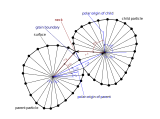
\includegraphics[height=78mm]{img/model_development/two_particle_contact}
\end{frame}

\section{Description of Contact Topology by Graphs}\label{sec:contact-graphs}

The contact topology of multiple particles can be described as a graph, where the vertices correspond to particles and the edges correspond to contact relations between the particles.
The undirected graph structure of a particle contact is shown in \autoref{fig:model_development/particle_graph}.
The indices of the vertices are at this point arbitrary, but are reused in the same way in the following.

For simulation purposes, the introduction of a hierarchy in the particle contacts is feasible to introduce a specific order for equation construction.
More specifically the particle contacts shall be described as a~\gls{DAG}.
Such a graph can always be constructed from a given undirected graph by performing a \gls{BFGS} starting at the desired root vertex and dropping all edges pointing back to the parent.
An example of such a structure in shown in \autoref{fig:model_development/particle_graph_dag}.
The particle labeled with index 0 is the \emph{root} of the graph, the only vertex that has no incoming edges.
In general, the root of the particle graph can be chosen arbitrarily, but for efficiency reasons, it should be a particle which leads to a graph as flat as possible.
The root particle has a fixed position in space and therefore acts as origin for all coordinate systems used throughout the calculations.
There may be cases, where the particle graph has rooted tree structure, which simplifies the problem significantly, since then all particles are able to move freely.
Edges like the red one in the figure break the tree structure.
Note, that they do not form cycles in the~\gls{DAG} in the meaning of graph theory, since the edges are directed.
But in terms of the underlying undirected graph they are anyway cycles.
To avoid ambiguities, the term ring contact shall be used here instead.
Ring contacts introduce additional constraints to the particle movement, since each particle in the ring influences the movement of the others.
The edges closing a ring are named correspondingly as \glspl{RCE}.

\begin{figure}
    \centering
    \includegraphics{img/model_development/particle_graph}
    \caption{Undirected Particle Graph Representing Contact Conditions}
    \label{fig:model_development/particle_graph}
\end{figure}

\begin{figure}
    \centering
    \includegraphics{img/model_development/particle_graph_dag}
    \caption{Directed Acyclic Graph Structure of Particle Contacts Rooted at Vertex 0}
    \label{fig:model_development/particle_graph_dag}
\end{figure}

\Glspl{RCE} are discovered during a~\gls{BFGS} when a vertex is encountered that was already marked as visited.
To be able to construct geometric constraints on particle movement, a ring path must be defined.
A ring path is a path following the cycle in the undirected graph, the currently regarded ring corresponds to.
It is generally not unique, but this is also not necessary.
To find a ring path, a~\gls{DFGS} is performed on the undirected particle graph with the ring closing edge removed.
The removed edge is afterwards appended to the path to close the ring.
The procedure is illustrated in \autoref{fig:model_development/particle_graph_ring_search}.

\begin{figure}
    \centering
    \includegraphics{img/model_development/particle_graph_ring_search}
    \caption{Ring Path Search Using a Depth-First Graph Search}
    \label{fig:model_development/particle_graph_ring_search}
\end{figure}


\chapter{Application of the Thermodynamic Extremal Principle}\label{ch:tep_application}

In the following the generalized extremal principle is applied on the current model of particles and nodes, see \autoref{subsubsec:extremal-priciple-generalized} for details on the approach.
As before, an index of the currently regarded particle or node is neglected where appropriate for brevity.
The indices $\ldots_{\Upper}$ and $\ldots_{\Lower}$ are used to denote the upper resp.~lower neighbor of a node.
${\Nodes}$ is the set of all nodes present in the system and ${\Particles}$ the set of all particles, respectively.

\section{Choice of Variables}\label{sec:variables}

First, the internal state variables $\Vect\InternalStateVariable$, the internal state velocities $\Vect\InternalStateVelocity$ and the fluxes $\Vect\Flux$ must be chosen.
The feasibility of the approach heavily depends on this choice.

The choice of the fluxes is straightforward with the diffusional fluxes.
One has two diffusional fluxes from each node $\Flux_{\Upper}$ and $\Flux_{\Lower}$ to the upper respectively the lower neighbor, however the flux of the upper node to the lower and the flux from the lower to the upper are always equal due to constancy of mass.
So in the following only $\Flux_{\Upper}$ shall be regarded and $\Flux_{\Lower}$ is substituted by $-\Flux_{\Upper}$ where necessary.

The internal state variables are the polar coordinates of the nodes $\left[ \Radius, \Angle \right]$ with pole in their particle's center, since they determine the thermodynamic forces and the main aim of the simulation is to follow the time evolution of the particles and nodes.
The coordinates of the particles $\left[ \X_{\Particle}, \Y_{\Particle} \right]$ are not used as internal state variables, since they are unambiguously defined, if the coordinates of all nodes relative to their particle are known and also which nodes are in contact to each other.
Moreover, the velocities of particle coordinates $\dot\X_{\Particle}$ and $\dot\Y_{\Particle}$ are auxiliary variables (included in $\Vect\AuxiliaryVariable$) to ease formulation of the geometric constraints.

For numerical and equation formulation reasons, the internal state velocities $\dot\Radius$ and $\dot\Angle$ are replaced by the velocities of node shift along normal and tangential surface vectors $\dot\Shift_{\Normal}$ and $\dot\Shift_{\Tangential}$.
As they are determined, translation into new coordinates is directly possible using the relations obtained in the following sections.

The external state variables (such as temperature $\Temperature$ and pressure $\Pressure$) are not considered in the following, since they are assumed constant.

\chapter{Equation System}\label{ch:equation-system}


\section{Components of the Lagrangian Gradient}\label{sec:components-of-the-lagrangian-gradient}

The following table displays all components of the Lagrangian gradient to be solved for the application of the \gls{TEP}.
Node symbols $n$ or contact symbols $c$ in parentheses behind another symbol mean, that this symbol is local to the node or contact, thus there exist one distinct value for each node or contact.
$n_\Upper$ denotes the upper neighbor of the currently regarded node, as well as $n_\Lower$ the lower.
The equations are all formulated in terms of fluxes from one node to the upper neighbor $\Flux_{\Upper}$, since $\Flux_\Lower(n) = -\Flux_\Upper(n_\Lower)$ must be always fulfilled.
This saves one unknown per node.

\begin{longtblr}[
    label=none,
    entry=none,
    note{*}={Only if the node is in parent position.}
]{
    colspec={lX[c]},
    measure=vbox
}
    \toprule
    \SetCell[c=2]{l} for each non-contact node $n$ \\
    \midrule
    $\LagrangeFunction_{\Step\Shift_\Normal(n)}$ &
    \begin{equation*}
        0
        = \frac{\partial\GibbsEnergy}{\partial\Shift_\Normal(n)} \left( 1 + \LagrangeParameter_1 \right)
        + \frac{\partial\Volume(n)}{\partial\Shift_\Normal(n)} \LagrangeParameter_{\Volume}(n)
    \end{equation*} \\

    $\LagrangeFunction_{\Flux_\Upper(n)}$ &
    \begin{equation*}
        0
        = \frac{2 \GasConstant \Temperature}{\MolarVolume \VacancyConcentration^\Standard} \frac{\SurfaceDistance_\Upper(n) \Flux_\Upper(n)}{\DiffusionCoefficient_\Upper(n)} \LagrangeParameter_1
        - \LagrangeParameter_\Volume(n)
        + \LagrangeParameter_\Volume(n_\Upper)
    \end{equation*} \\

    $\LagrangeFunction_{\LagrangeParameter_\Volume(n)}$ &
    \begin{equation*}
        0
        = \frac{\partial\Volume(n)}{\partial\Shift_\Normal} \Step\Shift_{\Normal}(n)
        - \Flux_{\Upper}(n)
        + \Flux_{\Upper}(n_\Lower)
    \end{equation*} \\

    \midrule
    \SetCell[c=2]{l} for each contact node $n$ as part of contact $c$ \\
    \midrule
    $\LagrangeFunction_{\Step\Shift_\Normal(n)}$ &
    \begin{equation*}
        0
        = \frac{\partial\GibbsEnergy}{\partial\Shift_\Normal(n)} \left( 1 + \LagrangeParameter_1 \right)
        + \frac{\partial\Volume(n)}{\partial\Shift_\Normal(n)} \LagrangeParameter_{\Volume}(n)
        - \frac{\partial \Radius_\Contact(c)}{\partial\Shift_\Normal(n)} \LagrangeParameter_{\Radius_\Contact}(n)
        - \frac{\partial \Angle_\Contact(c)}{\partial\Shift_\Normal(n)} \LagrangeParameter_{\Angle_\Contact}(n)
    \end{equation*} \\

    $\LagrangeFunction_{\Step\Shift_\Tangential(n)}$ &
    \begin{equation*}
        0
        = \frac{\partial\GibbsEnergy}{\partial\Shift_\Tangential(n)} \left( 1 + \LagrangeParameter_1 \right)
        + \frac{\partial\Volume(n)}{\partial\Shift_\Tangential(n)} \LagrangeParameter_{\Volume}(n)
        - \frac{\partial \Radius_\Contact(c)}{\partial\Shift_\Tangential(n)} \LagrangeParameter_{\Radius_\Contact}(n)
        - \frac{\partial \Angle_\Contact(c)}{\partial\Shift_\Tangential(n)} \LagrangeParameter_{\Angle_\Contact}(n)
    \end{equation*} \\

    $\LagrangeFunction_{\Flux_\Upper(n)}$ & same as above \\

    $\LagrangeFunction_{\LagrangeParameter_\Volume(n)}$ &
    \begin{equation*}
        0
        = \frac{\partial\Volume(n)}{\partial\Shift_\Normal} \Step\Shift_{\Normal}(n)
        + \frac{\partial\Volume(n)}{\partial\Shift_\Tangential} \Step\Shift_{\Tangential}(n)
        - \Flux_{\Upper}(n)
        + \Flux_{\Upper}(n_\Lower)
    \end{equation*} \\

    $\LagrangeFunction_{\LagrangeParameter_{\Radius_\Contact}(n)}$\TblrNote{*} &
    \begin{multline*}
        0
        = \Step\Radius_{\Contact}(c)
        - \frac{\partial \Radius_\Contact(c)}{\partial\Shift_\Normal(n)} \left( \Step\Shift_{\Normal}^{|\Parent}(n) + \Step\Shift_{\Normal}^{|\Child}(n) \right)
        - \frac{\partial \Radius_\Contact(c)}{\partial\Shift_\Tangential(n)} \left( \Step\Shift_{\Tangential}^{|\Parent}(n) + \Step\Shift_{\Tangential}^{|\Child}(n) \right) \\
        - 2 \frac{\partial \Radius_\Contact(c)}{\partial\Shift_\RotationAngle(n)} \Radius^{|\Child}(n) \sin \frac{\Step\RotationAngle_\Child(c)}{2}
    \end{multline*} \\

    $\LagrangeFunction_{\LagrangeParameter_{\Angle_\Contact}(n)}$\TblrNote{*} &
    \begin{multline*}
        0
        = \Step\Angle_{\Contact}(c)
        - \frac{\partial \Angle_\Contact(c)}{\partial\Shift_\Normal(n)} \left( \Step\Shift_{\Normal}^{|\Parent}(n) + \Step\Shift_{\Normal}^{|\Child}(n) \right)
        - \frac{\partial \Angle_\Contact(c)}{\partial\Shift_\Tangential(n)} \left( \Step\Shift_{\Tangential}^{|\Parent}(n) + \Step\Shift_{\Tangential}^{|\Child}(n) \right) \\
        - 2 \frac{\partial \Angle_\Contact(c)}{\partial\Shift_\RotationAngle(n)} \Radius^{|\Child}(n) \sin \frac{\Step\RotationAngle_\Child(c)}{2}
    \end{multline*} \\

    \midrule
    \SetCell[c=2]{l} for each contact $c$ with the therein involved nodes of the parent $\Nodes^{|\Parent}(c)$ \\
    \midrule
    $\LagrangeFunction_{\Step\Radius_\Contact(c)}$ &
    \begin{equation*}
        0
        = \sum^{\Nodes^{|\Parent}(c)}_n \LagrangeParameter_{\Radius_\Contact}(n)
    \end{equation*} \\

    $\LagrangeFunction_{\Step\Angle_\Contact(c)}$ &
    \begin{equation*}
        0
        = \sum^{\Nodes^{|\Parent}(c)}_n \LagrangeParameter_{\Angle_\Contact}(n)
    \end{equation*} \\

    $\LagrangeFunction_{\Step\RotationAngle_\Child(c)}$ &
    \begin{multline*}
        0
        = \sum^{\Nodes^{|\Parent}(c)}_n \Biggl[
            - \Radius^{|\Child}(n) \sin \left( \Step\RotationAngle_\Child(c) + \Angle^{|\Child}(n) - \Angle_\Contact^{|\Child}(c) \right) \LagrangeParameter_{\Radius_\Contact}(n) \\
            + \frac{\Radius^{|\Child}(n)}{\Radius_\Contact(c)} \cos \left( \Step\RotationAngle_\Child(c) + \Angle^{|\Child}(n) - \Angle_\Contact^{|\Child}(c)  \right) \LagrangeParameter_{\Angle_\Contact}(n)
            \Biggr]
    \end{multline*} \\

    \midrule
    \SetCell[c=2]{l} just once for the set of all nodes $\Nodes$ \\
    \midrule
    $\LagrangeFunction_{\LagrangeParameter_1}$ &
    \begin{equation*}
        0
        = \sum^\Nodes_n \left[
            \frac{\partial\GibbsEnergy}{\partial\Shift_\Normal(n)} \Step\Shift_\Normal(n)
            + \frac{\partial\GibbsEnergy}{\partial\Shift_\Tangential(n)} \Step\Shift_\Tangential(n)
            - \frac{\SurfaceDistance_\Upper(n) \Flux_\Upper(n)^2 + \SurfaceDistance_\Lower(n) \Flux_\Upper(n_\Lower)^2}{2\GasConstant\Temperature\MolarVolume\VacancyConcentration^\Standard}
            \right]
    \end{equation*} \\
    \bottomrule
\end{longtblr}


\section{Components of the Lagrangian Gradient's Jacobian}\label{sec:components-of-the-lagrangian-gradients-jacobian}
\section{Evolution of Particle Surfaces by Node Shifting}\label{sec:surface-evolution}

\begin{figure}
    \begin{subfigure}{\linewidth}
        \centering
        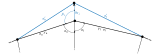
\includegraphics{img/model_development/node_shift_normal}
        \caption{Normal Direction}
        \label{fig:model_development/surface_normal}
    \end{subfigure}
    \begin{subfigure}{\linewidth}
        \centering
        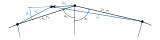
\includegraphics{img/model_development/node_shift_tangential}
        \caption{Tangential Direction}
        \label{fig:model_development/surface_tangential}
    \end{subfigure}
    \caption{Shifting of Surface Nodes}
    \label{fig:surface-node-shifting}
\end{figure}

\begin{figure}
    \begin{subfigure}{0.5\linewidth}
        \centering
        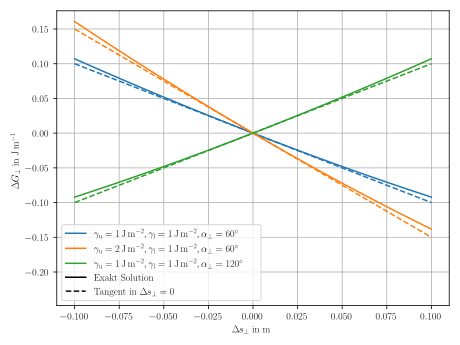
\includegraphics[scale=0.5]{img/model_development/plot_normal_potential}
        \caption{Normal Direction}
        \label{fig:model_development/plot_normal_potential}
    \end{subfigure}%
    \begin{subfigure}{0.5\linewidth}
        \centering
        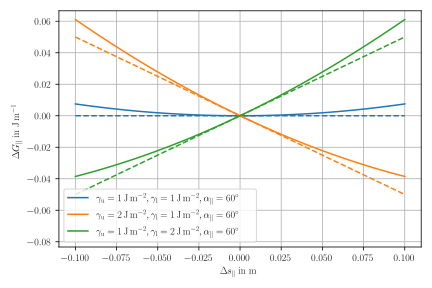
\includegraphics[scale=0.5]{img/model_development/plot_tangential_potential}
        \caption{Tangential Direction}
        \label{fig:model_development/plot_tangential_potential}
    \end{subfigure}
    \caption{Change in Gibbs Energy Due to Node Shifting (tangents dashed)}
    \label{fig:surface-node-potentials}
\end{figure}

In the following, the Gibbs energy and volume gradients when shifting nodes will be derived as needed in the formulation of dissipation $\Dissipation$ and dissipation function $\DissipationFunction$ given above.

\subsection{Normal Shifting}

The main mode of node shifting on free surfaces and grain boundaries is along the interface normal vector.
\autoref{fig:model_development/surface_normal} shows the principal geometry of a surface node and it's normal mode of shifting.

If a node is displaced in space, a change in Gibbs energy occurs due to the change in surface respectively interface area.
The amount of energy bound in a surface or interface is described by the interface energy $\InterfaceEnergy$.
Since a 2D problem is regarded, the length of the surface line $\SurfaceDistance$ is a measure of present surface area.
The change of Gibbs energy due to normal node shifting is described by \autoref{eq:gibbs-diff-surface-normal} with the prime values as measures after shifting.
\begin{equation}
    \Step\GibbsEnergy_{\Normal} = \left( \SurfaceDistance_{\Upper}' - \SurfaceDistance_{\Upper} \right) \InterfaceEnergy_{\Upper} +  \left(\SurfaceDistance_{\Lower}' - \SurfaceDistance_{\Lower} \right) \InterfaceEnergy_{\Lower}
    \label{eq:gibbs-diff-surface-normal}
\end{equation}

The normal vector points under an angle of $\SurfaceVectorAngle_\Normal$ acc.~to~\autoref{eq:delta-surface-normal} to both surface lines.
\begin{equation}
    \SurfaceVectorAngle_{\Normal} = \PI - \frac{1}{2} \left(\SurfaceRadiusAngle_{\Upper} + \SurfaceRadiusAngle_{\Lower} \right)
    \label{eq:delta-surface-normal}
\end{equation}

With a certain normal shift ${\Step\Shift}_\Normal$, the surface lengths after shifting are calculated by \autoref{eq:surface-distance-shifted-normal}.
\begin{subequations}
    \begin{align}
        \SurfaceDistance_{\Upper}' & = \sqrt{\SurfaceDistance_{\Upper}^2 + \Step\Shift_{\Normal}^2 - 2 \SurfaceDistance_{\Upper} \Step\Shift_{\Normal} \cos \SurfaceVectorAngle_{\Normal}} \label{eq:surface-distance-shifted-normal-upper}         \\
        \SurfaceDistance_{\Lower}' & = \sqrt{{\SurfaceDistance}_{\Lower}^2 + {\Step\Shift}_{\Normal}^2 - 2 {\SurfaceDistance}_{\Lower} {\Step\Shift}_{\Normal} \cos \SurfaceVectorAngle_{\Normal}} \label{eq:surface-distance-shifted-normal-lower}
    \end{align}
    \label{eq:surface-distance-shifted-normal}
\end{subequations}

\autoref{fig:model_development/plot_normal_potential} shows the change in Gibbs energy due to normal shifting with use of \autoref{eq:gibbs-diff-surface-normal} to \autoref{eq:surface-distance-shifted-normal} with different values of $\SurfaceVectorAngle_{\Normal}$ and $\InterfaceEnergy$, alongside the linear approximation around ${\Step\Shift}_{\Normal} = 0$.
Note, that the slope is dependent on the sum of ${\InterfaceEnergy}_{\Upper}$ and ${\InterfaceEnergy}_{\Lower}$ and the sign is only dependent on $\SurfaceVectorAngle_{\Normal}$.
$\SurfaceVectorAngle_{\Normal} > \qty{90}{\degree}$ means a convex surface, thus energy gain when inward shifting (negative ${\Step\Shift}_{\Normal}$).
$\SurfaceVectorAngle_{\Normal} < \qty{90}{\degree}$ means a concave surface, thus energy gain when outward shifting (positive ${\Step\Shift}_{\Normal}$).
$\SurfaceVectorAngle_{\Normal} = \qty{90}{\degree}$ means an even surface, thus energy loss in both shifting directions.

The partial derivative of Gibbs energy is obtained as the limit of $\Step\GibbsEnergy_{\Normal}$ when ${\Step\Shift}_{\Normal} \rightarrow 0$ as in \autoref{eq:gibbs-partial-surface-normal}.
\begin{equation}
    \frac{\partial \GibbsEnergy}{\partial {\Shift}_{\Normal}} = \lim_{\Step\Shift_{\Normal} \rightarrow 0} \frac{\Step\GibbsEnergy_{\Normal}}{\Step\Shift_{\Normal}} = -\left({\InterfaceEnergy}_{\Upper} + {\InterfaceEnergy}_{\Lower}\right) \cos \SurfaceVectorAngle_{\Normal}
    \label{eq:gibbs-partial-surface-normal}
\end{equation}

The volume derivative is obtained by calculating the area of the triangles formed by $\SurfaceDistance$, $\SurfaceDistance'$ and $\Step\Shift_{\Normal}$ on the upper and lower side.
\begin{subequations}
    \begin{align}
        \Step\Volume_{\Normal\Upper} &= \frac12 \SurfaceDistance_{\Upper} \Step\Shift_{\Normal} \sin \SurfaceVectorAngle_{\Normal} \\
        \Step\Volume_{\Normal\Lower} &= \frac12 \SurfaceDistance_{\Lower} \Step\Shift_{\Normal} \sin \SurfaceVectorAngle_{\Normal}
    \end{align}
    \label{eq:volume-diff-surface-normal}
\end{subequations}

The partial derivative of volume is obtained as the limit of $\Step\Volume_{\Normal\Upper} + \Step\Volume_{\Normal\Lower}$ when ${\Step\Shift}_{\Normal} \rightarrow 0$ as in \autoref{eq:volume-partial-surface-normal}.
\begin{equation}
    \frac{\partial \Volume}{\partial {\Shift}_{\Normal}} = \lim_{\Step\Shift_{\Normal} \rightarrow 0} \frac{\Step\Volume_{\Normal\Upper} + \Step\Volume_{\Normal\Lower}}{\Step\Shift_{\Normal}} = \frac{1}{2} \left( \SurfaceDistance_{\Upper} + \SurfaceDistance_{\Lower} \right) \sin \SurfaceVectorAngle_{\Normal}
    \label{eq:volume-partial-surface-normal}
\end{equation}

\subsection{Tangential Shifting}

Regarding the tangential shifting, the direction vector is under an angle of $\SurfaceVectorAngle_{\Tangential}$ acc.~to.~\autoref{eq:delta-surface-tangential} to the upper surface line.
\begin{equation}
    \SurfaceVectorAngle_{\Tangential} = \SurfaceVectorAngle_{\Normal} - \frac{\PI}{2}
    \label{eq:delta-surface-tangential}
\end{equation}

The change in Gibbs energy is calculated similarly as in the normal case according to \autoref{eq:gibbs-diff-surface-tangential}, but the shifted surface lengths are calculated as in \autoref{eq:surface-distance-shifted-tangential} in dependence on the tangential shift ${\Step\Shift}_{\Tangential}$.
Note especially the signs in front of the cosine terms.
\begin{equation}
    \Step\GibbsEnergy_{\Tangential} = \left( \SurfaceDistance_{\Upper}' - \SurfaceDistance_{\Upper} \right) \InterfaceEnergy_{\Upper} +  \left(\SurfaceDistance_{\Lower}' - \SurfaceDistance_{\Lower} \right) \InterfaceEnergy_{\Lower}
    \label{eq:gibbs-diff-surface-tangential}
\end{equation}
\begin{subequations}
    \begin{align}
        \SurfaceDistance_{\Upper}' & = \sqrt{{\SurfaceDistance}_{\Upper}^2 + {\Step\Shift}_{\Tangential}^2 - 2 {\SurfaceDistance}_{\Upper} {\Step\Shift}_{\Tangential} \cos \SurfaceVectorAngle_{\Tangential}} \label{eq:surface-distance-shifted-tangential-upper} \\
        \SurfaceDistance_{\Lower}' & = \sqrt{{\SurfaceDistance}_{\Lower}^2 + {\Step\Shift}_{\Tangential}^2 + 2 {\SurfaceDistance}_{\Lower} {\Step\Shift}_{\Tangential} \cos \SurfaceVectorAngle_{\Tangential}} \label{eq:surface-distance-shifted-tangential-lower}
    \end{align}
    \label{eq:surface-distance-shifted-tangential}
\end{subequations}

\autoref{fig:model_development/plot_tangential_potential} shows the change in Gibbs energy due to tangential shifting with different values of $\InterfaceEnergy$.
The slope and monotonicity of these curves is here dependent on the \emph{difference} of ${\InterfaceEnergy}_{\Upper}$ and ${\InterfaceEnergy}_{\Lower}$.
The convexity or concavity of the surface is here only of minor importance.
Whether the interface with higher $\InterfaceEnergy$ is located on the upper or lower side determines the monotonicity of the curves.
In the special case when ${\InterfaceEnergy}_{\Upper} = {\InterfaceEnergy}_{\Lower}$, the curve has a minimum in ${\Step\Shift}_{\Tangential} = 0$, meaning that any shift will produce an energy loss.
This is the case on all nodes except neck nodes.

Again, the partial derivative of Gibbs energy is found by the limit when ${\Step\Shift}_{\Tangential} \rightarrow 0$.
\begin{equation}
    \frac{\partial \GibbsEnergy}{\partial {\Shift}_{\Tangential}} = \lim_{\Step\Shift_{\Tangential} \rightarrow 0} \frac{\Step\GibbsEnergy_{\Tangential}}{\Step\Shift_{\Tangential}} = -\left({\InterfaceEnergy}_{\Upper} - {\InterfaceEnergy}_{\Lower}\right) \cos \SurfaceVectorAngle_{\Tangential}
    \label{eq:gibbs-partial-surface-tangential}
\end{equation}

The partial derivative of volume is found similarly as in the normal case, but the contribution of the lower side must be here counted negatively, as can be seen from \autoref{fig:model_development/surface_tangential}.
\begin{equation}
    \frac{\partial \Volume}{\partial {\Shift}_{\Tangential}} = \lim_{\Step\Shift_{\Tangential} \rightarrow 0} \frac{\Step\Volume_{\Tangential\Upper} - \Step\Volume_{\Tangential\Lower}}{\Step\Shift_{\Tangential}} = \frac{1}{2} \left( \SurfaceDistance_{\Upper} - \SurfaceDistance_{\Lower} \right) \sin \SurfaceVectorAngle_{\Tangential}
    \label{eq:volume-partial-surface-tangential}
\end{equation}

\subsection{Special Treatment of Neck Nodes}

\begin{figure}
    \begin{subfigure}{\linewidth}
        \centering
        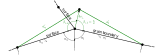
\includegraphics{img/model_development/node_shift_normal_neck}
        \caption{Normal Direction}
        \label{fig:model_development/node_shift_normal_neck}
    \end{subfigure}
    \begin{subfigure}{\linewidth}
        \centering
        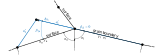
\includegraphics{img/model_development/node_shift_tangential_neck}
        \caption{Tangential Direction}
        \label{fig:model_development/node_shift_tangential_neck}
    \end{subfigure}
    \caption{Shifting of Neck Nodes}
    \label{fig:surface-node-shifting-neck}
\end{figure}

The neck nodes (triple points between two surfaces and one grain boundary) are a special case.
For numerical reasons, their shifting is not taken normal and tangential to the surface line, but only to the grain boundary, as this is in consistence with their primary evolution during sintering.
The case, where the grain boundary is located below the currently regarded node, is shown in \autoref{fig:surface-node-shifting-neck}.
Here, one must distinguish between the shift vector angles $\SurfaceVectorAngle$ to the upper and the lower surface line.
For the shown case the angles are as in \autoref{eq:shift-neck-angles}, if the grain boundary is, however, located above the node, than the values of the upper and lower angles have to be switched.
\begin{align}
    \SurfaceVectorAngle_{\Normal\Upper} = \frac32 \PI - \SurfaceRadiusAngle_{\Upper} - \SurfaceRadiusAngle_{\Lower} \qquad &\text{and} \qquad \SurfaceVectorAngle_{\Normal\Lower} = \frac\PI2 \\
    \SurfaceVectorAngle_{\Tangential\Upper} = \PI - \SurfaceRadiusAngle_{\Upper} - \SurfaceRadiusAngle_{\Lower} \qquad &\text{and} \qquad \SurfaceVectorAngle_{\Tangential\Lower} = 0
    \label{eq:shift-neck-angles}
\end{align}

The respective partial derivatives are slightly modified with the distinct angles as below.
\begin{align}
    \frac{\partial \GibbsEnergy}{\partial {\Shift}_{\Normal}} &= -\left( {\InterfaceEnergy}_{\Upper} \cos \SurfaceVectorAngle_{\Normal\Upper} - {\InterfaceEnergy}_{\Lower} \cos \SurfaceVectorAngle_{\Normal\Lower} \right)
    \label{eq:gibbs-partial-neck-normal} \\
    \frac{\partial \Volume}{\partial {\Shift}_{\Normal}} &= \frac{1}{2} \left( \SurfaceDistance_{\Upper} \sin \SurfaceVectorAngle_{\Normal\Upper} + \SurfaceDistance_{\Lower} \sin \SurfaceVectorAngle_{\Normal\Lower}\right)
    \label{eq:volume-partial-neck-normal} \\
    \frac{\partial \GibbsEnergy}{\partial {\Shift}_{\Tangential}} &= -\left( {\InterfaceEnergy}_{\Upper} \cos \SurfaceVectorAngle_{\Tangential\Upper} - {\InterfaceEnergy}_{\Lower} \cos \SurfaceVectorAngle_{\Tangential\Lower}\right)
    \label{eq:gibbs-partial-neck-tangential} \\
    \frac{\partial \Volume}{\partial {\Shift}_{\Tangential}} &= \frac{1}{2} \left( \SurfaceDistance_{\Upper} \sin \SurfaceVectorAngle_{\Tangential\Upper} - \SurfaceDistance_{\Lower} \sin \SurfaceVectorAngle_{\Tangential\Lower}\right)
    \label{eq:volume-partial-neck-tangential}
\end{align}

\section{Contact Conditions Between Particles}\label{sec:contact-conditions}

\begin{figure}
    \centering
    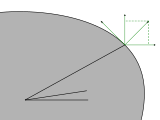
\includegraphics{img/model_development/node_shift_global}
    \caption{Geometric Conditions for Global Node Displacement}
    \label{fig:model_development/node_shift_global}
\end{figure}

In contrast to free surfaces, where the geometric evolution of a node is not constrained by the surrounding space, in grain boundaries the node shifting acts counter the solid material of the other particle.
This introduces additional constraints, since the grain boundary must not form voids and must not overlap.
The geometric constraints are dependent on the local evolution of the grain boundary nodes, as well as the relative position change of the particles.

Starting from a compact grain boundary, meaning that there are no holes and/or overlap present within it, the condition of maintaining the compactness of the grain boundary can be formulated as follows, if the postions of the particles are fixed.
\begin{subequations}
    \begin{align}
        \Step\Shift_{\Normal}\Regarding1 = \Step\Shift_{\Normal}\Regarding2 \\
        \Step\Shift_{\Tangential}\Regarding1 = \Step\Shift_{\Tangential}\Regarding2
    \end{align}
    \label{eq:maintain-compact-particles-fixed}
\end{subequations}

But in reality the positions of particles to each other change, which can be observed macroscopically as shrinkage.
So we formulate instead the total displacement of a node in absolute cartesian space, which must be equal regarded from both particles.
The total node displacement includes contributions from particle displacement (index $\Particle$), normal node displacement (index $\Normal$) and tangential node displacement (index $\Tangential$).
\begin{subequations}
    \begin{align}
        \Step\X_{\Particle1} + \Step\X_{\Normal}^{\Regarding1} + \Step\X_{\Tangential}^{\Regarding1} + \Step\X_{\RotationAngle}^{\Regarding1}
        &= \Step\X_{\Particle2} + \Step\X_{\Normal}^{\Regarding2} + \Step\X_{\Tangential}^{\Regarding2} + \Step\X_{\RotationAngle}^{\Regarding2}\\
        \Step\Y_{\Particle1} + \Step\Y_{\Normal}^{\Regarding1} + \Step\Y_{\Tangential}^{\Regarding1} + \Step\Y_{\RotationAngle}^{\Regarding1}
        &= \Step\Y_{\Particle2} + \Step\Y_{\Normal}^{\Regarding2} + \Step\Y_{\Tangential}^{\Regarding2} + \Step\Y_{\RotationAngle}^{\Regarding2}
        \label{eq:absolute-displacement-contact-constraints}
    \end{align}
\end{subequations}

As can be seen from \cref{fig:model_development/node_shift_global}, the angles of projection of the normal and tangential node shifting to the global cartesian axes are as follows:
\begin{subequations}
    \begin{align}
        \eta_{\Normal} &= \RotationAngle + \Angle + \left( \SurfaceRadiusAngle_{\Lower} + \SurfaceVectorAngle_{\Normal\Lower} - \PI \right)
        \label{eq:global-shift-normal-angle} \\
        \eta_{\Tangential} &= \left( \PI - \SurfaceRadiusAngle_{\Lower} + \SurfaceVectorAngle_{\Tangential\Lower} \right) - \RotationAngle - \Angle
        \label{eq:global-shift-tangential-angle}
    \end{align}
\end{subequations}

With these and further identities on the trigonometric functions the displacements of the node are given as follows:
\begin{subequations}
    \begin{align}
        \Step\X_{\Normal} &= -\Step\Shift_{\Normal} \cos \left( \RotationAngle + \Angle + \SurfaceRadiusAngle + \SurfaceVectorAngle \right)
        \label{eq:global-shift-normal-x} \\
        \Step\Y_{\Normal} &= -\Step\Shift_{\Normal} \sin \left( \RotationAngle + \Angle + \SurfaceRadiusAngle + \SurfaceVectorAngle \right)
        \label{eq:global-shift-normal-y} \\
        \Step\X_{\Tangential} &= \Step\Shift_{\Tangential} \cos \left( \RotationAngle + \Angle + \SurfaceRadiusAngle + \SurfaceVectorAngle \right)
        \label{eq:global-shift-tangential-x} \\
        \Step\Y_{\Tangential} &= \Step\Shift_{\Tangential} \sin \left( \RotationAngle + \Angle + \SurfaceRadiusAngle + \SurfaceVectorAngle \right)
        \label{eq:global-shift-tangential-y}
    \end{align}
\end{subequations}

Inserted in \cref{eq:absolute-displacement-contact-constraints} this leads to two additional constraints for each contact node (grain boundary or neck node), which define the particle displacements $\Step\X_{\Particle i}$ and $\Step\Y_{\Particle i}$ of each particle except one.
Given one grain boundary node (only normal displacement allowed) and two neck nodes per contact, the equation system is unambiguously defined as we have 6 additional constraints (2 per node) for 2 particle displacements and 4 tangential neck node displacements.
Introducing more grain boundary nodes creates more constraints but no additional unknowns (as their normal displacement and flux are covered by the volume balance respectively the optimization).
This leads to an overdetermined system which forces the solution to zero shrinkage (contact nodes are not able to be displaced at all).
Also allowing the grain boundary nodes to be displaced tangentially, leads to an underdetermined system as the contact conditions are not able to determine the particle position anymore.
A solution to this issue has not been found at the time writing this work, so the following applications will be restricted to two neck nodes and one grain boundary node per particle per contact.
This also forbids multiple contacts between the same particles, which is impossible for circular particle geometries but may be for arbitrarily shaped ones.


\chapter{Software Implementation of the Model}\label{ch:implementation}

Reference to open source code

\section{Representation of Particles and Nodes}\label{sec:representation}
\begin{itemize}
    \item Classes
    \item Tree Structure
    \item Coordinate Systems
\end{itemize}

\section{Numerical Solution Procedure}\label{sec:solution}

\subsection{Time Integration Scheme}\label{subsec:time-integration-scheme}

The time integration scheme follows a simple explicit Eulerian forward procedure.
This method, however, is prone to numerical instabilities, which are often observed as alternating zick-zack like surface structures (see \autoref{sec:numerical-behavior}).
Therefore, the time step width must be limited.
As the normal or tangential displacements of a node in one step are bad measures due to the varying distances between the nodes, it was chosen to use the surface angles (which are a measure for curvature) as indicator for time step width.

The angle difference is calculated in accordance to the equations in \autoref{sec:surface-evolution} with $\Step\Shift = \dot\Shift \Step\Time$.

\begin{equation}
    \max_i^{\Nodes} \max_j^{[\Upper, \Lower]} \max_k^{[\Normal, \Tangential]} \arcsin \left( \frac{\SurfaceDistance}{\SurfaceDistance'} \sin \SurfaceVectorAngle_{jk} \right)  < \qtyrange{0.01}{0.1}{\radian}
    \label{eq:maximum-angle-difference}
\end{equation}

\subsection{Step System Solution}\label{subsec:step-system-solution}

The application of the \gls{TEP} leads to a non-linear system of equations, although most equations are linear therein with a few exceptions, most notably the main dissipation equality constraint.
The system size is dependent on the count of particles present in the simulation and the count of points defining their surface.
Typically, it contains from a few hundred to a few thousands of components.
Solution of this system is accomplished using the standard Newton method, as this method is known for fast convergence thus sparing evaluations of the system.
This method requires the evaluation of the systems gradient resp.~it's Jacobian matrix, which is sparse and follows the general structure shown in \autoref{fig:implementation/sparse_structure}.
The complete set of components for the Jacobian are given in \autoref{sec:components-of-the-lagrangian-gradients-jacobian}.
Newton's method is, however, also known for its vulnerability to the choice of the initial solution estimation (see \autoref{subsubsec:solution-estimation}).
As the regarded system only includes linear, bilinear and quadratic terms, non-convergence does not have to be expected here.
However, the system may have two solutions caused by the quadratic terms, so the procedure may converge to the wrong one.

Most notably, in a particle system without external loads, the trivial solution (overall dissipation is zero) is a valid solution of the equation system, but the minimum of dissipation rather its maximum.
During testing, it has been noticed that in cases where the solution procedure converges to the trivial solution, doubling the initial solution estimate often pushes the procedure to converge to the right solution.
This is a simple and fast trick to avoid this issue.
The reasoning behind this is, that the overall dissipation at necks is often underestimated by the step estimator.
Convergence to the trivial solution usually occurs, when the estimated overall dissipation is to small by several orders of magnitude.

The calculation of a Newton step requires the solution of the linear system in \autoref{eq:newton-step}, where $J_{\LagrangeFunction}$ is the Jacobian of the Lagrangian and $\Grad \LagrangeFunction$ it's gradient.
The system is solved in each step by LU-factorization using an algorithm specialized for sparse matrices of \textcite{Davis2006} implemented in the CSparse.NET package \textcite{Woltering2024}.

\begin{equation}
    J_{\LagrangeFunction}(x) \cdot \Step x = -\Grad \LagrangeFunction(x)
    \label{eq:newton-step}
\end{equation}

\begin{figure}
    \centering
    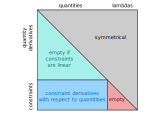
\includegraphics[scale=0.6]{img/implementation/sparse_structure}
    \caption{General Structure of the Systems Jacobian Matrix}
    \label{fig:implementation/sparse_structure}
\end{figure}

\subsubsection{Solution Estimation}\label{subsubsec:solution-estimation}

The estimation of the step solution is a crucial point to ensure fast and reliable convergence of the Newton procedure.

The solution on free surfaces is easily obtained with high precision by first estimating the vacancy concentrations using \autoref{eq:vacancy-concentration}, but expressing the chemical potential by the Gibbs energy gradient of \autoref{eq:gibbs-partial-surface-normal} as in \autoref{eq:chemical-potential-by-gibbs-gradient}.

\begin{equation}
    \Estimated{\Diff\ChemicalPotential} = \frac{\partial\GibbsEnergy}{\partial\Step_{\Normal}} \cdot \frac{2\MolarVolume}{\SurfaceDistance_{\Upper} + \SurfaceDistance_{\Lower}}
    \label{eq:chemical-potential-by-gibbs-gradient}
\end{equation}

Then the fluxes are obtained using Fick's first law (\autoref{eq:fick-first}).
By balancing the fluxes and dividing by the volume gradient, the normal displacement of a node is obtained:

\begin{equation}
    \Estimated{\Step\Shift_{\Normal}} = \left( \Flux_{\Upper} - \Flux_{\Lower} \right) \left( \frac{\partial\Volume}{\partial\Shift_{\Normal}} \right)^{-1}
    \label{eq:estimate-normal-displacement}
\end{equation}

When simulating the evolution of a single particle free in space, this estimate solves the step directly.
A single Newton step is than only needed to obtain the Lagrange multipliers.
When, however, a sinter neck is present, the situation becomes much more complicated, as the neck points feature two modes of displacement with distinct volume and energy gradients and the requirement of maintaining contact.
The issue is solved using a fixed-poit iteration procedure, whose starting point is the simple estimation described above.
The target variable is the flux between the neck node and the central grain boundary node, denoted here as $\Estimated\Flux$.

In the first approximation, the normal displacement of the neck nodes must be equal to that of the grain boundary node to fulfill contact consitions.
Then, the tangetial displacement of the neck node calculates as in \autoref{eq:estimate-neck-tangetial-displacement} using the flux balance there, with $\Flux_{\Surface}$ as the estimated flux to the adjacent surface node calculated as above and $i$ as the iteration index.

\begin{equation}
    \Estimated{\Step\Shift_{\Tangential i}} =
    \left( \Estimated{\Flux_i} - \Flux_{\Surface} - \frac{\partial\Volume}{\partial\Shift_{\Normal}} \Estimated{\Step\Shift_{\Normal i}} \right)
    \left( \frac{\partial\Volume}{\partial\Shift_{\Tangential}} \right)^{-1}
    \label{eq:estimate-neck-tangetial-displacement}
\end{equation}

With this the total dissipation on the neck node is given by:

\begin{equation}
    \Estimated{\Dissipation_i}
    = \frac{\partial\GibbsEnergy}{\partial\Shift_{\Normal}} \Estimated{\Step\Shift_{\Normal i}}
    + \frac{\partial\GibbsEnergy}{\partial\Shift_{\Tangential}} \Estimated{\Step\Shift_{\Tangential i}}
    \label{eq:estimated-neck-dissipation}
\end{equation}

Using the form of the dissipation function in \autoref{eq:dissipation-function-node} the new flux is obtained as in \autoref{eq:estimated-neck-new-flux}.
The signum term is required to support negative dissipations, which occur when the system reaches a stationary state of the surface near the neck in later stages which is characterized by small fluctuations.

\begin{equation}
    \Estimated{\Flux_{i+1}} =
    \sign \Estimated{\Dissipation_i} \cdot
    \sqrt{
        \frac{\MolarVolume{\VacancyConcentration}^\Standard}{\GasConstant\Temperature}
        \frac{\DiffusionCoefficient_{\Upper}}{\SurfaceDistance_{\Upper}}
        \Abs{\Estimated{\Dissipation_i}}
    }
    \label{eq:estimated-neck-new-flux}
\end{equation}

This flux is then inserted in the iteration again in \autoref{eq:estimate-normal-displacement} for the grain boundary nodes and \autoref{eq:estimate-neck-tangetial-displacement} for the neck node till the fixed point is reached.

\section{Calculation and Extraction of Key Features}\label{sec:extraction}
\begin{itemize}
    \item Volume Cell, Shrinkage
    \item Neck Measures
\end{itemize}



\part{Model Application and Validation}\label{part:model-application-and-validation}
\chapter{Investigation of the Model's Numerical Behavior}\label{ch:numerical-behavior}

\section{Study on Remeshing Influence}\label{sec:remeshing_study}

\chapter{Investigation of the Model's Physical Behavior}\label{ch:physical-behavior}

\section{Study on the Influence of Key Physical Parameters}

The simulation of an asymmetrical two-particle-contact involves a variety of physical geometry and material parameters which highly influence the sintering behavior and macroscopic response of the system to be observed.
A widely used approach to characterize a system is by it's dimensionless parameters.
The following study investigates the influence of the dimensionless parameters present in an asymmetrical two-particle-system.

\subsection{Construction of the Study}

The shape of a particle is here modeled as an ellipse an parameterized with the equivalent circular radius $\Radius_{\Particle}$ and the ovality $\Ovality \in [ 1, \infty ) $ (as the standard eccentricity is an hardly illustrative value for the current purpose).
The local polar radius coordinate of a node is then given by \autoref{eq:parameter_study_ellipse_function}, with the main radii defined by $a = \Radius_{\Particle} \sqrt{\Ovality}$ and $b = \Radius_{\Particle} / \sqrt{\Ovality}$ with $a/b = o$.

\begin{equation}
    \Radius(\Angle) = \frac{a b}{\sqrt{\left( a \sin \Angle \right)^2 + \left( b \cos \Angle \right)^2  }}
    \label{eq:parameter_study_ellipse_function}
\end{equation}

\begin{table}
    \caption{Investigated Dimensionless Parameters and their Range}
    \label{tab:parameter_study_conditions}
    \begin{tblr}{colspec={lrrlX}, row{1}={l}}
        \toprule
        Parameter & Min & Max & Scale & remarks \\
        \midrule
        $\Radius_1 / \Radius_2$ & \num{1} & \num{10} & log & equal material\\
        $\DiffusionCoefficient_{\GrainBoundary} / \DiffusionCoefficient_{\Surface} $ & \num{0.01} & \num{1} & log & equal material\\
        $\InterfaceEnergy_{\GrainBoundary} / \InterfaceEnergy_{\Surface}$ & \num{0.01} & \num{1} & log & equal material \\
        $\DiffusionCoefficient_{2} / \DiffusionCoefficient_{1} $ & \num{1} & \num{100} & log \\
        $\InterfaceEnergy_{2} / \InterfaceEnergy_{1}$ & \num{1} & \num{10} & log \\
        $o$ & \num{1} & \num{4} & log & tip/tip contact \\
        $o$ & \num{1} & \num{4} & log & tip/flank contact \\
        $o$ & \num{1} & \num{4} & log & flank/flank contact \\
        \bottomrule
    \end{tblr}
\end{table}

\subsection{Discussion of the Results}

The results will be displayed as isoline-plots for shrinkage and neck size with the normalized time on the horizontal axis and the regarded dimensionless parameter on the vertical axis.

\section{Study on the Influence of Multiple Particle Contacts}

\subsection{Construction of the Study}

\subsection{Discussion of the Results}


\chapter{Randomized Simulation of Particle Packings}\label{ch:randomized-simulations}

In the previous chapter the numerical and physical behavior of the model was analysed.
Thereby, the transition from a two-particle-model to a multi-particle-model was performed.
The results of \autoref{sec:contact-study} show, that the effects of pore closure can be incoporated by investigating a particle arrangement of at least three particles.
The sintering behavior of all investigated arrangements was the same except for the region where the pore is almost closed.
Also, the effects of multi-material contacts can be regarded.
In the following investigation, the particle arrangement shall be randomized using statistically generated particles as developed in \autoref{ch:statistical-powder-modeling}.

\section{Construction of the Study}

The study will stick to three-particle arrangements to avoid major difficulties in construction of the initial state.
As the size and shape of the particles will now be variable, the initial position can not be given a-priori but must be determined numerically.
The study will compare three cases: three powders with equal particle size distribution but one assumed to have circular particles,
one where only an ovality according to \autoref{eq:f-ovality} is considered
and one where also first order waves according to \autoref{eq:f-first-order-waves} are considered.
The differences and similarities of the three cases will be investigated to rate the need for inclusion of this data into sintering simulations.
The core question is if the first order waves have major influence or if regard on ovality is enough, since ovality is a parameter that can be measured without problems using state of the art automatic particle classifiers.
First order waves, however, require an high amount of manual work.
The author has already published a paper describing a method to obtain these for aggregate particles via laser scanning microscopy images and leat-square fitting in \textcite{Weiner2022a}, but there an another approach of sintering model is used.

\subsection{Statistical Description of the Example Powder}

The values used in this study do not represent a real powder, but are crafted to illustrate the procedure and reveal the influence of the particle shape counter classic circular shapes.
The results will be normalized as was done in the previous studies, so the distributions in the following are designed to support this.

The particle size distribution for all powders is taken as a Weibull distribution (\autoref{eq:weibull-particle-size}) with expectation $\Expectation(\Radius_0)$, which will be used as the reference radius to calculate the characteristic time norm according to \autoref{eq:normalized_time}.
The shape parameter $k$ is taken as \num{3.602} to achieve a non-skewed distribution.
Then, the scale parameter $\lambda$ can directly be obtained from the expectation as given below.
$\Gamma$ is the gamma function.
\begin{equation}
    \Probability(\Radius_0) = \lambda k (\lambda \Radius_0)^{k-1} \exp -(\lambda \Radius_0)^k \qquad \text{with} \qquad \lambda = \frac{\Gamma(1+\frac1k)}{\Expectation(\Radius_0)}
    \label{eq:weibull-particle-size}
\end{equation}

The ovality is modeled using an exponential distribution which is shifted by \num{1} and has the expectation $\Expectation{\Ovality}= \num{1.5}$:
\begin{equation}
    \Probability(\Ovality)  = \frac{1}{\lambda} \exp -\lambda \left( \Ovality - 1 \right) \qquad \text{with} \qquad \lambda = \frac{1}{\Expectation(\Ovality) - 1}
    \label{eq:exponential-ovality}
\end{equation}

The wave height is modeled using a beta distribution:\todo{Explain reasoning of distribution choice.}
\begin{equation}
    \Probability(\WaveHeight) = \frac{1}{\Beta(\alpha, \beta)} \WaveHeight^{\alpha - 1} \left( 1 - \WaveHeight \right) ^ {\beta - 1}
    \label{eq:beta-wave-height}
\end{equation}

\subsection{Creation of the Initial State}

The intial state generation starts by sampling three particles randomly.
For each a radius $\Radius_0$ and one of every shape parameter is sampled from the given distribution.
Also, the rotation of each particle is sampled from a uniform distribution with value range $\RotationAngle \in [0, 2\PI)$.
The initial position of the particles is created in enough distance to each other, so that it is impossible for them to be in contact.

The first particle is kept fixed in space.
Then, the second is moved along the vector towards the center of the first in small steps until contact is created by a defined minimum intersection of the two surfaces.
Then the third is moved along the sum of of the vectors from the thirds center to the others' centers.
If contact with one is created, then the vector towards this particle is counted negative to allow sideward movement.
When the third particle has contact to both, the procedure is completed.

\section{Discussion of the Results}

\todo{Add and discuss results. (Simulation not conducted yet.)}

\chapter{Conclusions and Outlook}\label{ch:conclusions-and-outlook}

A novel approach to model sintering behavior of two or multiple particles in 2D space has been developed which supports asymmetric geometry and substance conditions.
The approach uses sharp interfaces and a finite difference approximation of the particle surfaces.
The model was based on the \gls{TEP} to obtain a concise and flexible formulation of the evolution equations.
The model allows direct identification of physical interface properties due to the sharp interface formulation.
Additional requirements such as contact conditions are to be formulated as equality constraints an can be implicitly ensured by the solution procedure.

The numerical behavior of the model has been examined to define feasible parameters for numerical routines such as time step control and remeshing procedures.
The computational effort for time integration of the model equation can be heavily lowered by feasible time step control and rigorous remeshing procedures.
In early stages of the simulation remeshing has to be done with care to keep the fine details of geometry, in later stages however remeshing can be aggressive to reduce the system size and accelerate the solution procedure.
The latter is an significant improvement counter state-of-the-art \gls{PFM} approaches, which usually have larger system sizes in general and may not reduce the system size during the simulation.
Although remeshing procedures are applied there, too, the discretization sizes are determined by the phase field gradient requirements, rather than the interface geometry as in the current case.
So in the current case the requirements on discretization fineness decrease during the simulation, where in \gls{PFM} they do not.

The model has then be used to conduct extensive parameter studies on two-particle configurations.
The varied parameters include classic ones like the ratio of surface energy to grain boundary energy or the ratio of surface and grain boundary diffusion rate, for which previous results have been confirmed and the new model has been validated.
Other parameters, for which no previous results could be found in literature, have been investigated regarding the influence of asymmetric substance pairings and particle geometries.
As validation against findings from the literature was not possible here, explanations of the observed behavior have been attempted.

In a third step, the behavior of powder mixtures has been investigated by simulating the sintering of random arrangements of three particles.
\todo{Conclude about randomized simulations.}

\begin{figure}
    \includegraphics{img/conclusions/shrinkage_influences}
    \caption{Influence of Dimensionless Parameters and Packing Properties on Shrinkage Summarized from Investigations in This Work}
    \label{fig:conclusions/shrinkage_influences}
\end{figure}

\begin{figure}
    \includegraphics{img/conclusions/neck_size_influences}
    \caption{Influence of Dimensionless Parameters and Packing Properties on Neck Size Evolution Summarized from Investigations in This Work}
    \label{fig:conclusions/neck_size_influences}
\end{figure}

The dimensionless parameter studies, as well as the investigations of crafted and random packings have lead to several general statements about the influence on shrinkage and neck size evolution during sintering.
The results are summarized graphically in \autoref{fig:conclusions/shrinkage_influences} for the shrinkage and \autoref{fig:conclusions/neck_size_influences} for the neck size.

In the current state of the model, several incompletenesses have been observed during the investigations conducted:
\begin{enumerate}
    \item Triple points where three grain boundaries meet are currently not supported.
        This limits the applicability till the closing of the first pore present in the system.
    \item In contacts between particles with high difference in surface energy, a drastic undercut near the neck occurs as discussed in \autoref{subsec:parameter-study-asymmetric-surface-energy-ratio},
        which eventually leads to a crossing between grain boundary and surface, which is obviously unphysical.
        This is an numerical effect due to the removal of volume from a node, where in fact no volume is left.
    \item The grain boundary can currently only consist of a single node (plus the two neck nodes) as was discussed in \autoref{sec:contact-conditions},
        as otherwise the contact conditions create collinear rows in the system matrix.
    \item Transfer between particles was neglected, which disallowed the occurrence of grain growth in the parameter studies of asymmetric geometry (\autoref{subsec:parameter-study-particle-size-ratio} and \autoref{subsec:parameter-study-ovality}),
        but allowed to disregard concentration gradients within the particle volume for the case of unequal substances.
\end{enumerate}

Beside fixing those, further development of the model can include in the future:
\begin{enumerate}
    \item Introduction of an multi-scale approach that models fine-grained powder fractions as a solid continuum of viscoelastic behavior filling the pores with ability to apply a pressure on the large particles' surfaces and transfer mass to them.
    \item Transfer the approach for simulation of microstructure evolution of compact polycrystals regarding recrystallization, but also possibly with phase transformations.
\end{enumerate}


\addpart{References}
\printunsrtglossary[type=\glsxtrabbrvtype,title=List of Abbreviations]
% tex-fmt: off
\addchap{List of Symbols}

\begin{longtblr}[
    label=none,
    entry=none,
]{lX}
    \toprule
    Symbol               & Meaning              \\
    \midrule
    
      ${}{{ symbol.value }}{}$ & {{ symbol.comment }} \\
    
    \bottomrule
\end{longtblr}

\listoffigures
\listoftables

\printbibliography

\end{document}
